\section{Experimental Evaluation}
\label{sec:experiments}
To understand the trade-offs between these Distribution Strategies (DSs), we perform four sets of experiments using queries over target families presented on the GtoPdb website. The first set of experiments use real queries extracted from citations to GtoPdb published in the British Journal of Pharmacology.  
The second set uses synthetically produced provenance polynomials, corresponding to more complex queries, in order to better highlight the differences between the DSs.
The third set of experiments considers the accrual of credit over time by the three strategies, again using synthetic queries.
The fourth set of experiments shows how the DSs compare to traditional citations in giving credit to data curators using both real and synthetic queries.
%We close by discussing the relative execution times of the three strategies.

%All experiments were carried out on a MacBook Pro %13-inch, 2019 
%with a 2.4 GHz processor Intel Core i5 quad-core and 8 GB of memory at 2133 MHz.  
The source code for the experiments is written in Java and supported by a PostgreSQL database. For purposes of reproducibility, the code we used for our experiments and all queries are available here: \url{https://bitbucket.org/dennis_dosso/credit_distribution_project}.

\subsection{Real-world queries}
\label{sec:real_world_queries}

\begin{figure}[t]
\centering
  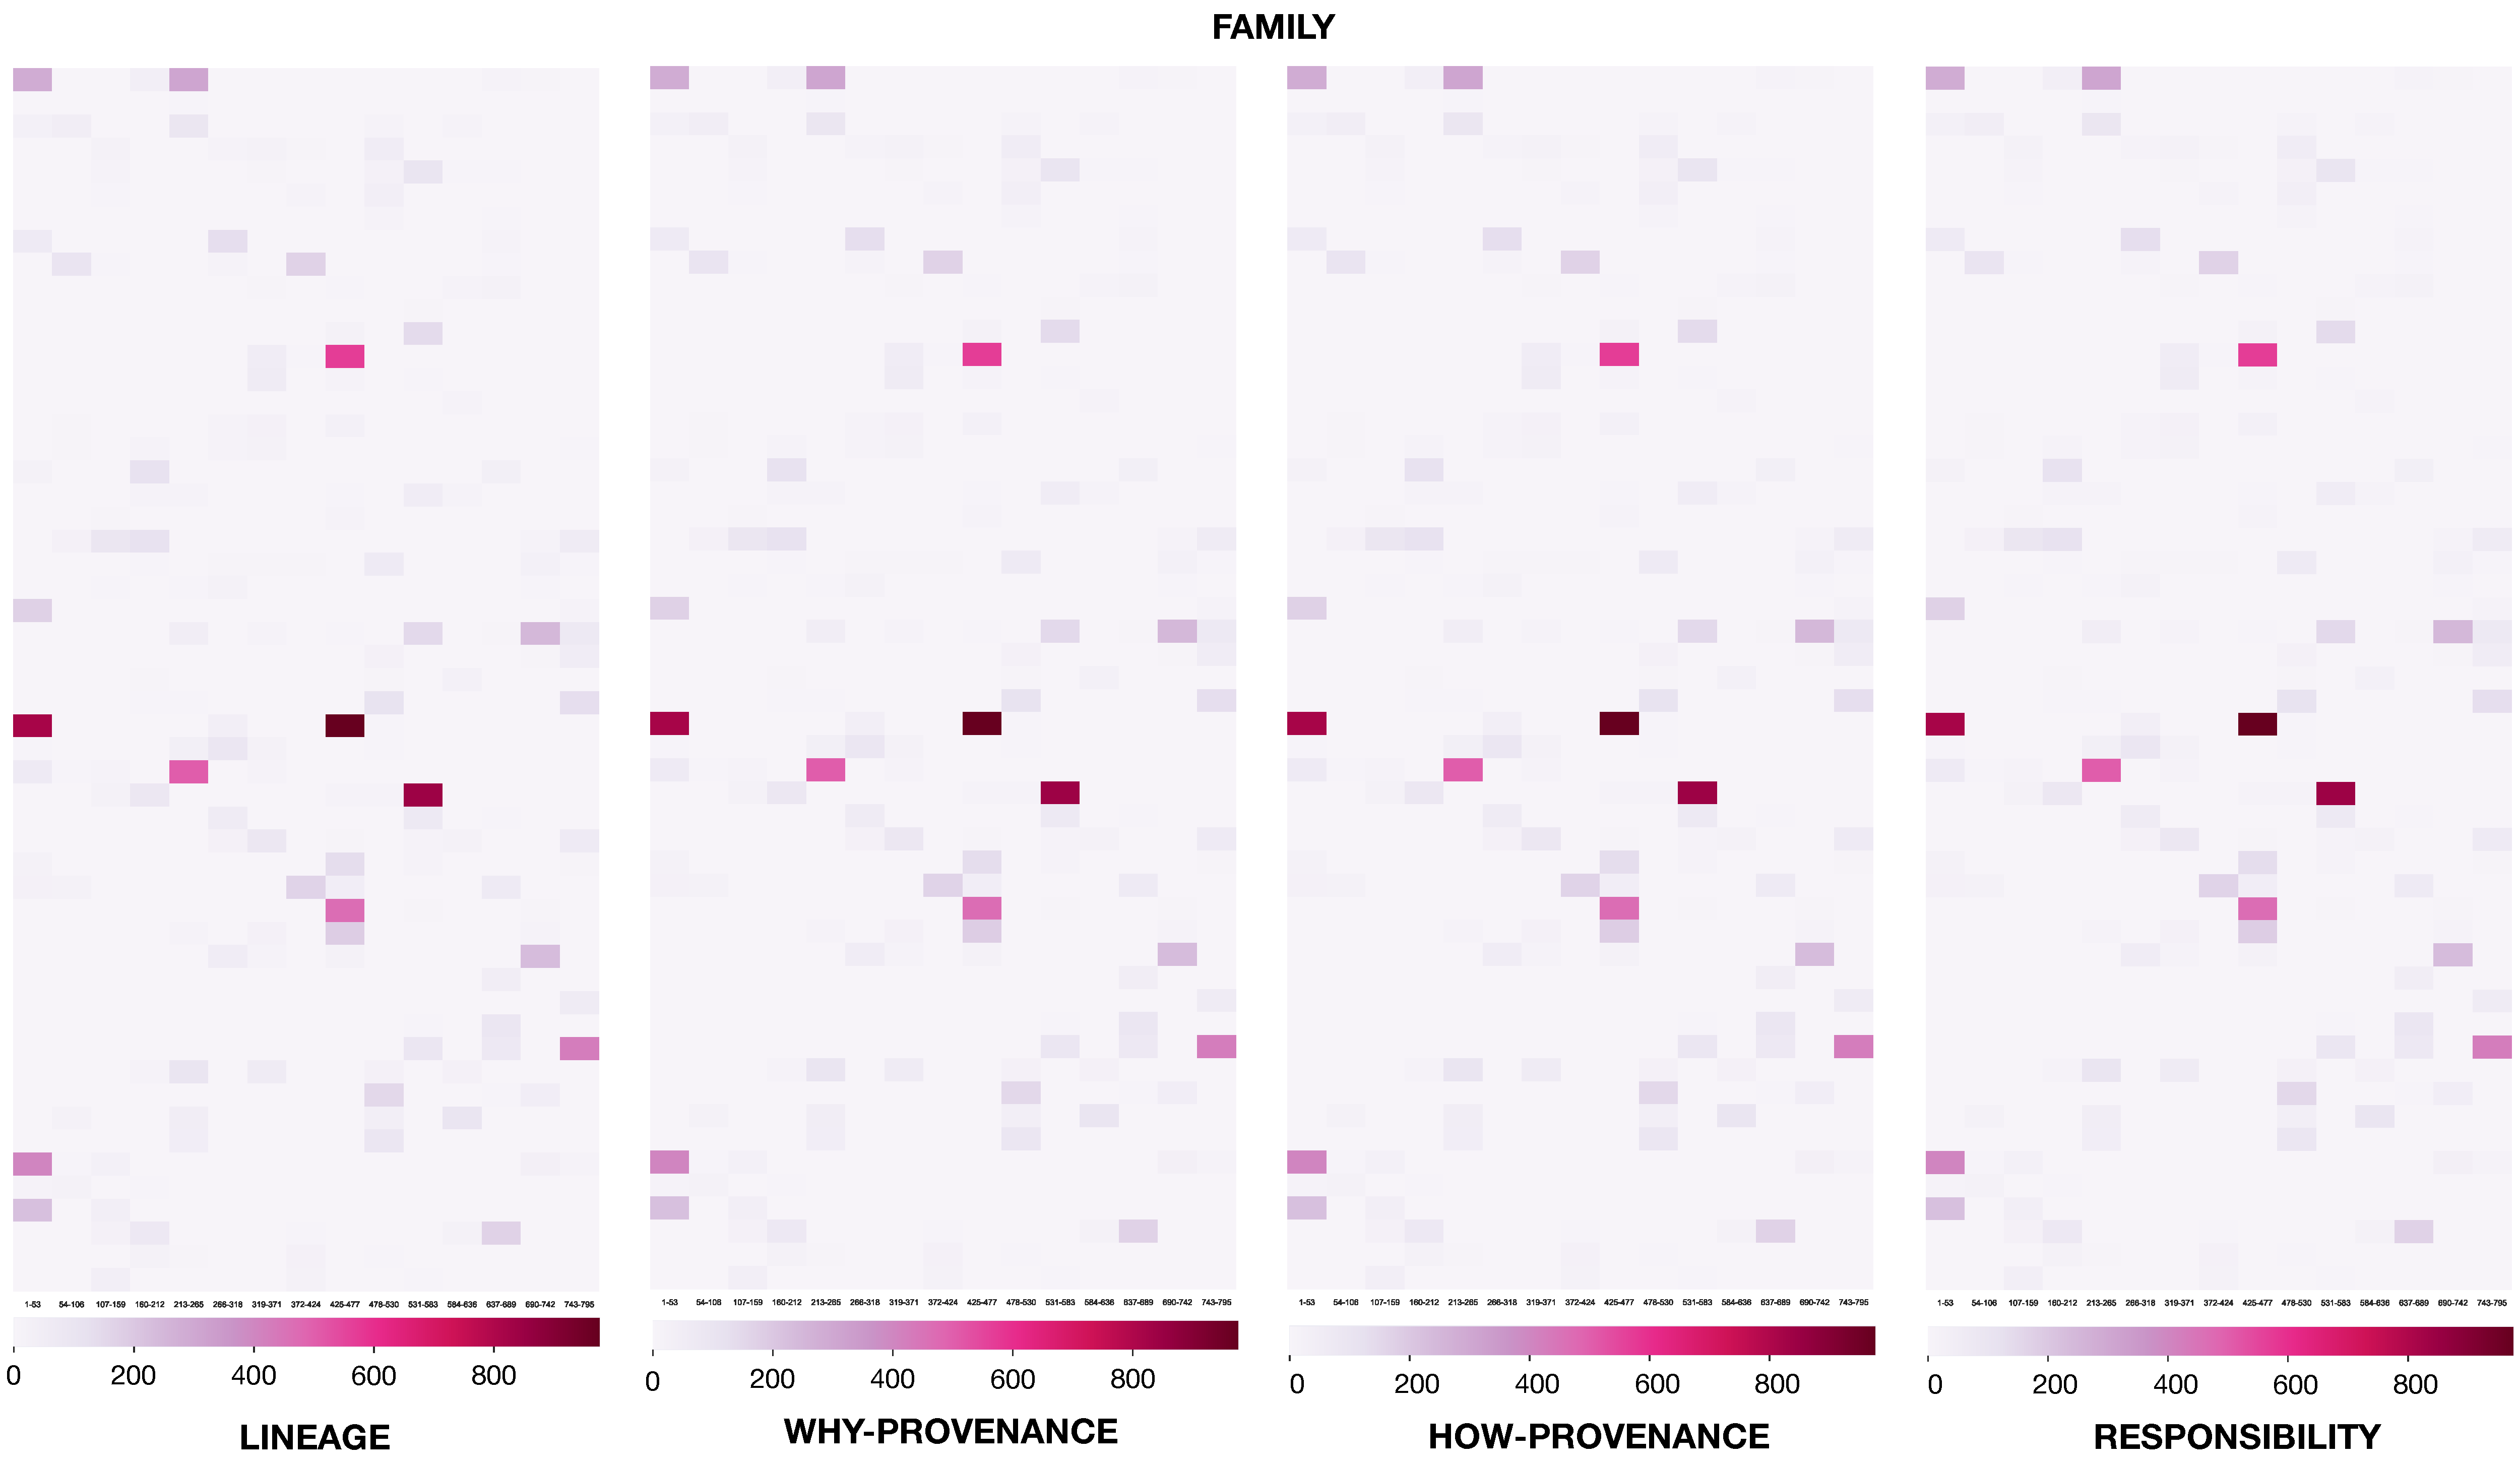
\includegraphics[width=\textwidth]{figures/paper_based}
  \caption{Comparison of four DS on the same table \texttt{family} using the distribution given by the queries retrieved from papers. Each cell is a tuple.}
  \label{figure:comparison_on_papers}
\end{figure}


%We evaluate the proposed distribution strategies on GtoPdb, and in particular, we focus on target families described on the GtoPdb website. 

%When a paper uses data from GtoPdb, it can cite the full database, a webpage of interest, or a subset of data extracted with a query. 

Examples of real queries are drawn from papers published in the British Journal of Pharmacology (BJP)~\footnote{\url{https://bpspubs.onlinelibrary.wiley.com}}.  Each time a paper in this journal cites a webpage from GtoPdb, it reports the URL of the page. From this URL, the query used to obtain the webpage data can be determined. 
We considered all $889$ papers in BJCP citing the IUPHAR/BPS Guide to pharmacology \citep{iuphar2018} as of October 2020, and extracted all webpage URLs to GtoPdb contained within the paper.\footnote{The IUPHAR/BPS Guide is a journal that describes the structure and evolution of GtoPdb. At the time of writing, it had received more than $1200$ citations on Google Scholar.}

\eat{
There are eight target family webpages linked from the GtoPdb website: \emph{GPCR}, \emph{Ion channels}, \emph{NHRs}, \emph{Kinases}, \emph{Catalytic receptors}, \emph{Transporters}, \emph{Enzymes} and \emph{Other protein targets}.}
The queries that we inferred are those used to build target family webpages within GtoPdb.
An example was given in Figure \ref{figure:family_structure}, where we show how the structure of the ``Adenosine receptors'' family can be mapped into  queries over the underlying database. %to get the information reported in the corresponding webpage. 
In GtoPdb, all target family pages share a similar structure; the only difference is that individual sections, such as ``contributors'' or ``further readings'', may be missing.
Therefore, the same queries can be used to build all of the target family pages by changing the family id used in the query (for example, in Figure \ref{figure:family_structure}, it is 3).
Note that the queries are fairly simple SQL queries, and fall into a class called ``select-project-join" or ``SPJ" queries. 
A total of more than $12K$ different queries were built in this way.
Without loss of generality, we give each tuple in the output of a query a credit of $1$.

\paragraph{Results} Figure \ref{figure:comparison_on_papers} shows the heat-maps obtained by the distribution of credit according to the \rtwo{five} DS on one of the tables in the underlying database, \texttt{family}, 
%describes the characteristics and necessary information of the receptor families and, as can be seen in Figure \ref{figure:family_structure}, it 
which is often joined with other tables in the database to build the webpages. Each cell in a heat-map represents a tuple of the \texttt{family} table and the color indicates the amount of credit attributed to such tuple.
It can be seen that the result of  credit distribution over \texttt{family} is the same for all \rtwo{five} strategies. The same result is also obtained with the other tables of the database used by the queries shown in Figure \ref{figure:family_structure}. 

The reason why credit distribution is the same for all \rtwo{five} strategies is that the queries are all simple SPJ queries, which use each table only once and do joins on key attributes. 
Under these conditions, each tuple of the output presents: (i) a how-provenance that is a single monomial with coefficient one and exponent one in each variable; (ii) a why-provenance with only one witness; (iii) a lineage that is the same of the witness in the basis, \rtwo{(iv) all tuples are counterfactual causes when considering responsibility, and (v) all tuple have the same importance in the production of the output tuples according to their Shapley value}.
Hence, for these queries, the \rtwo{five} DSs behave in the same way: credit is uniformly distributed among the tuples of the lineage. 

To illustrate this, consider one of the queries in Figure \ref{figure:family_structure} which is used to build the output webpage:

\vspace{2mm}
{\footnotesize
\begin{adjustwidth}{25pt}{5pt}
	\begin{verbatim}
	Q3: SELECT c.first_names, c.surname
	FROM contributor2family AS cf JOIN contributor AS c ON 
	cf.contributor_id = c.contributor_id 
	WHERE f.family_id = 3
\end{verbatim}
\end{adjustwidth}
}
\vspace{2mm}

\texttt{Q3} returned $10$ tuples from the version of GtoPdb used. 
The first tuple, \texttt{<Bertil B., Fredholm>}, has  $c_{939} \cdot c2f_{496}$ as its provenance polynomial.
$c_{939}$ represents the provenance token of a tuple in \texttt{contributor}, and $c2f_{496}$ the provenance token of a tuple in table \texttt{contributor2family}. 
The why-provenance of this tuple is $\{\{c_{939}, cf_{496} \}\}$, its lineage is $\{c_{939}, c2f_{496} \}$, \rtwo{both these tuples are counterfactual causes and have a responsibility of one.}
Therefore, the credit assigned to these tuples is $1/2$ using all five DS.
This happens for all the tuples in the output of each query of GtoPdb, thus making the distributions equivalent over all outputs.

However, this is not the case with more complex queries. As we showed in the previous section, when two or more tuples are merged as a result of a projection or union, the credit distributions will differ between the strategies. %These are represented as multiple witnesses and multiple monomials. 

\begin{comment}
	
To give an example of how the CDS can differ from one another in their behavior, let us consider a different query:

\vspace{2mm}
{\footnotesize
\begin{adjustwidth}{25pt}{5pt}
	\begin{verbatim}
	Q4: SELECT f.name AS name
	FROM family AS F JOIN
	(SELECT DISTINCT f.family_id, f.name
	FROM "family" AS f JOIN contributor2family AS cf ON 
	f.family_id = cf.family_id 
	JOIN contributor c ON 
	cf.contributor_id = c.contributor_id 
	WHERE c.country = 'UK') AS R 
	ON F.name = R.name
\end{verbatim}
\end{adjustwidth}
}
\vspace{2mm}

Here the innermost query retrieves all the names and ids of the families written by an author from the UK producing a relation called $R$. This relation is then joined with the table \texttt{family} on the attribute \texttt{name}. 

One output tuple of this query is \texttt{<Histamine receptors>}, that has the following provenance polynomial:

{\footnotesize
\[
\begin{array}{c}
	f_{625}(f_{625} c2f_{656} c_{184} + f_{625} c2f_{113} c_{180} + f_{625} c2f_{283} c_{198} +\\ 
	+ f_{625} c2f_{550} c_{865} + f_{625} c2f_{573} c_{101} + f_{625} c2f_{95} c_{109} )
\end{array}
\]
}

As already discussed, the different monomials represent possible \emph{alternatives} of combinations of tuples that produce the considered output tuple. 
Tuple $f_{625}$ is used multiple times with different joins, thus it appears in each monomial. 
The last join, performed in the outmost query, is responsible for the final multiplication of $f_{625}$ with the rest of the polynomial between parenthesis.

From this polynomial we compute the why-provenance as a set of six different witnesses:

{\footnotesize
\[
\begin{array}{c}
\{\{ f_{625}, c2f_{656}, c_{184} \}, \{ f_{625}, c2f_{113}, c_{180} \} 
\{ f_{625}, c2f_{283}, c_{198} \}, \\ \{ f_{625}, c2f_{550}, c_{865} \},
 \{ f_{625}, c2f_{573}, c_{101}\} , \{f_{625}, c2f_{95}, c_{109} \}\}	\\
\end{array}
\]
}

And corresponding lineage:
{\footnotesize
\[
\begin{array}{c}
	\{ f_{625}, c2f_{656}, c_{184}, c2f_{113}, c_{180}, 
  c2f_{283}, c_{198}, c2f_{550}, c_{865}, 
  c2f_{573}, c_{101}, c2f_{95}, c_{109}\}
\end{array}
\]
}

\begin{figure}[tb]
  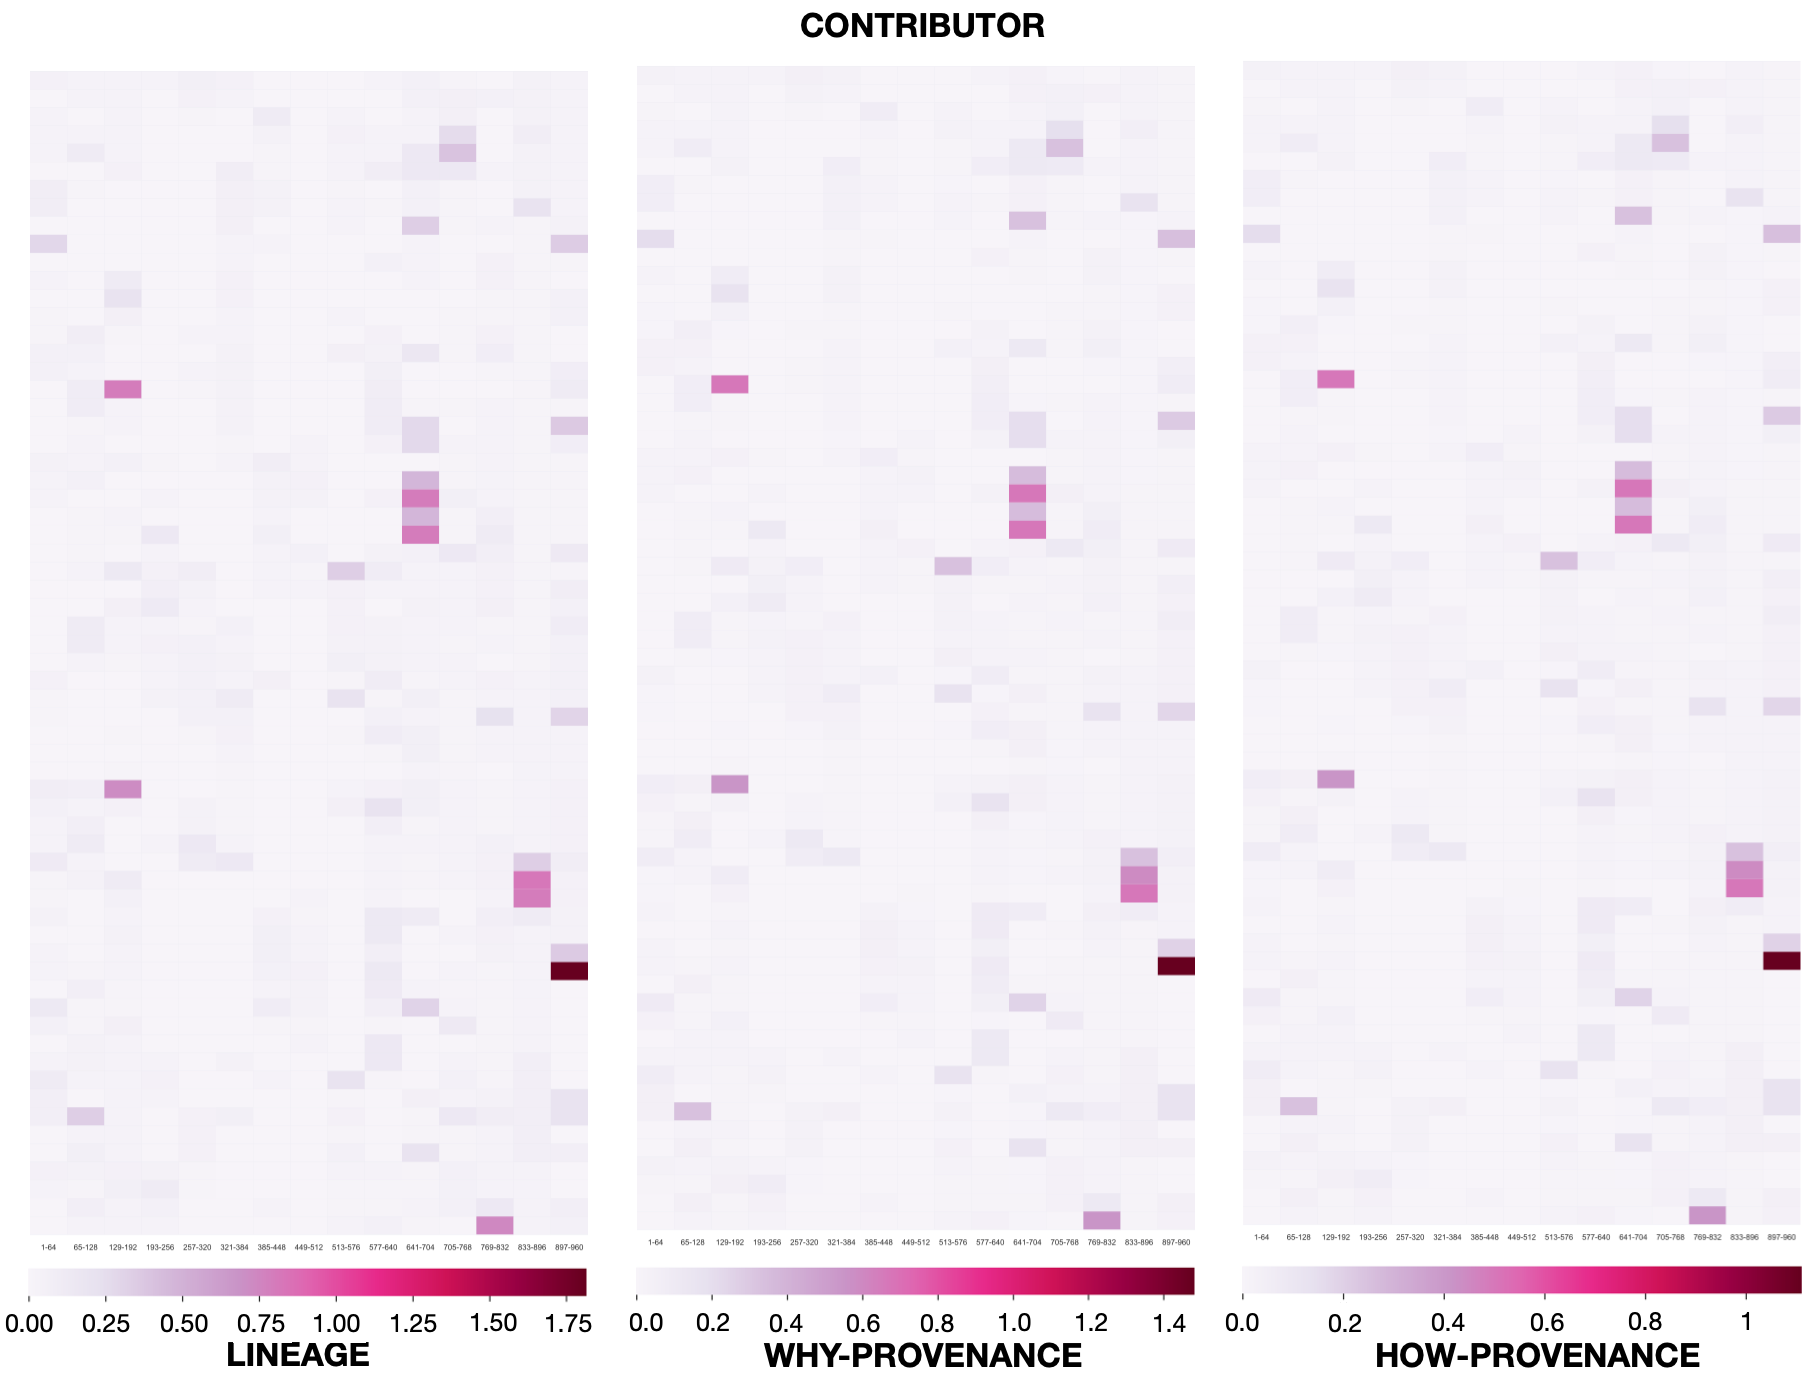
\includegraphics[width=1\textwidth]{figures/synthetic_queries}
  \caption{Comparison of three DS on the same table \texttt{family} after the distribution of the credit connected to query \texttt{Q4}.}
  \label{figure:comparison_on_synthetic_query_1}
\end{figure}

This was only one tuple among the $86$ obtained from this query. If we assign credit $1$ to all these tuples and distribute it with the different strategies, we obtain the result shown in Figure \ref{figure:comparison_on_synthetic_query_1} for the table \texttt{contributor}.
At first sight, it may appear that the three distributions produce the same result. This is only partially true: the heat maps appear equal, but the absolute values assigned to each tuple are different. 
This is more evident if we look at the legend of each heat-map, where the maximum quantity of credit is different for each distribution. The one performed through lineage is around $1.8$, the why-provenance's one is around $1.4$, and the one based on how-provenance is around $1.1$. 

To understand what is happening with this query in this specific table, consider the output tuple \texttt{<Histamine receptors>} and its provenances, as discussed above.
Let us focus on its lineage. There are a total of six authors for this family and $13$ tuples in total in the lineage. 
Thus, using the lineage-based DS, each tuple belonging to the \texttt{contributor} table (i.e. $c_{184}, c_{180}, c_{198}, c_{865}, c_{101}, c_{109}$) receives credit equal to $1/13$.
Tuple $f_{625}$ too receives a portion of credit equal to $1/13$.

Let us consider now why-provenance. Tuple $f_{625}$ appears six times in six different witnesses composed of $3$ elements each. From each witness it receives a portion of credit equal to $1/18$, thus its total credit is $1/3$.
On the other hand, all the authors appear only once in each witness, thus each of them receives credit $1/18$. 
In this case, why-provenance is recognizing more credit to tuple $f_{625}$, since it appears in each witness. The consequence is that this distribution is equally \emph{subtracting} credit from the other tuples in the witnesses and giving it to $f_{625}$. 
In Figure \ref{figure:comparison_on_synthetic_query_1} we are only looking at table \texttt{contributor}. 
This same effect is reproduced for each tuple of the output of query \texttt{Q4}, thus the \emph{absolute} credit values on the tuples vary depending on the deployed strategy. 
What happens is that the tuples in table \texttt{contributor} receive less credit than the one received using lineage, but in the same proportions. The heat map appears thus equal to the one obtained with lineage.
This same effect is also present with the how-provenance-based CDS. In this case, tuple $f_{625}$ is rewarded even more, since it appears with an exponent 2 in each monomial, thus attracting even more credit. 

This is also why when we look at the legend for each part of Figure \ref{figure:comparison_on_synthetic_query_1}, the maximum value reached with the lineage-based DS is higher than the one reached with the why-provenance-based DS, which in turn is higher than the one obtained with the how-provenance. This is because the different strategies reward less and less the tuples of table \texttt{contributor} and more the ones in table \texttt{family}. 

This clearly shows the ability of the different strategies to adapt to situations. All three of them can highlight the relevant tuples in the table. However, they differ in the way they reward the tuples. 
Depending on the task, one provenance can be preferred to the other. 
If the only interest is to highlight the relevant tuples, lineage is sufficient. 
If the interest is also to reward more the tuples that are fundamental to the output, one can also choose why- or how-provenance, knowing that how-provenance rewards even more than why-provenance the relevant tuples that are indispensable for the output.  

\end{comment}


\subsection{Synthetic queries}
\label{sec:synth_queries}
\eat{
let us consider the case reported in Figure \ref{figure:comparison_on_synthetic_polynomials_2}. 
The figure reports a distribution of credit performed on the table \texttt{family} through the generation of 10K \emph{synthetic} polynomials. 
We randomly generated provenance polynomials that might be the how-provenance of randomly generated synthetic queries, using the three GtoPdb tables \texttt{family}, \texttt{contributor2family}, and \texttt{contributor}. 
An example of a synthetic polynomial that will be used throughout this subsection is:
}

To see what happens with more complex queries, 
%highlight the differences between the three DS, 
\rone{we synthetically generated provenance polynomials in which the coefficients and exponents could be greater than one, and picked them at random from a uniform distribution.}
%that might be the how-provenance of randomly generated synthetic queries, 
The queries involve three GtoPdb tables: \texttt{family}, \texttt{contributor2family}, and \texttt{contributor}. 
\rone{The polynomials were generated as follows: first, the number of monomials was decided by  randomly choosing a number between one and six.  Then, we randomly chose a tuple from the  \texttt{family} table, one from the \texttt{contributor2family} table and one from the \texttt{contributor} table; these are the variables of the monomial. We then chose a coefficient for the monomial (between one and three) and an exponent for each tuple (between one and four). For the next monomial, we decided if we wanted to keep the same tuple from the table family as first tuple of the new monomial. To do so, we generated a random float number between zero and one. If the number was above $0.2$, we changed the family tuple.}

An example can be found in Figure~\ref{fig:syntheticDistributions}, which shows a sample synthetic provenance polynomial (the how-provenance), the corresponding why-provenance, lineage, \rtwo{the causality of the tuples of the lineage, together with their responsibility, and, finally, the Shapley values of the lineage tuples}.  The resulting credit distribution for each DS is also shown.

\begin{figure}
{\footnotesize{\bf How-provenance:}
$
3 f_1^3 c2f_1^2 c_1^2 + 2 f_1 c2f_2^3 c_2^3 + 4 f_5 c2f_{17}^4 c_{18}^3
$ }\\
\hspace{0.5in} 
{\footnotesize{\bf Credit distribution:}\\ $f_1 = \frac{59}{315}, f_5 = \frac{1}{18}, c2f_1 = \frac{2}{21}, c2f_2 = \frac{2}{15}, 
c2f_{17}=\frac{2}{9} , c_1 = \frac{2}{21}, c_2 = \frac{2}{15}, c_{18} = \frac{1}{6} 
$
}
\\
\\
{\footnotesize{\bf Why-provenance:}
$
\{ \{f_1, c2f_1, c_1\}, \{f_1, c2f_2, c_2\}, \{ f_5, c2f_{17}, c_{18}\} \}
$ 
}
\\
{\footnotesize{\bf Credit distribution:}\\
$
f_1 = \frac{2}{9}, f_5 = \frac{1}{9}, c2f_1 = \frac{1}{9}, c2f_2 = \frac{1}{9}, 
c2f_{17}=\frac{1}{9} , c_1 = \frac{1}{9}, c_2 = \frac{1}{9}, c_{18} = \frac{1}{9} 
$
}
\\
\\
{\footnotesize{\bf Lineage: }
$
\{f_1, f_5, c2f_1, c2f_2, c2f_{17}, c_1, c_2, c_{18} \}
$}
\\
{\footnotesize{\bf Credit distribution:}\\
$
f_1 = \frac{1}{8}, f_5 = \frac{1}{8}, c2f_1 = \frac{1}{8}, c2f_2 = \frac{1}{8}, 
c2f_{17}=\frac{1}{8} , c_1 = \frac{1}{8}, c_2 = \frac{1}{8}, c_{18} = \frac{1}{8} 
$}
\\
\\
{\footnotesize{\bf \rtwo{Causality:}}
\rtwo{counterfactual causes: $\emptyset$,\\
actual causes: $\{f_1, f_5, c2f_1, c2f_2, c2f_{17}, c_1, c_2, c_{18} \}$} \\
\rtwo{\textbf{Responsibility:}\\ 
$
f_1 = \frac{1}{2}, f_5 = \frac{1}{2}, c2f_1 = \frac{1}{3}, c2f_2 = \frac{1}{3}, 
c2f_{17}=\frac{1}{2} , c_1 = \frac{1}{3}, c_2 = \frac{1}{3}, c_{18} = \frac{1}{2}  
$
}}
\\
\rtwo{{\footnotesize{\bf Credit distribution:}\\
$
f_1 = \frac{3}{20}, f_5 = \frac{3}{20}, c2f_1 = \frac{1}{10}, c2f_2 = \frac{1}{10}, 
c2f_{17}=\frac{3}{20} , c_1 = \frac{1}{10}, c_2 = \frac{1}{10}, c_{18} = \frac{3}{20}  
$
}}
\\
\\
\rtwo{{\footnotesize{\bf Shapley value:}\\
$
f_1 = 0.258\bar{3}, f_5 = \frac{1}{8}, c2f_1 = 0.091\bar{6}, c2f_2 = 0.091\bar{6}, 
c2f_{17}=\frac{1}{8} , c_1 = 0.091\bar{6}, c_2 = 0.091\bar{6}, c_{18} = \frac{1}{8}  
$
}}

\caption{\rtwo{Sample synthetic provenance polynomial (how-provenance) and corresponding why-provenance, lineage, responsibility, and Shapley values, together with the corresponding credit distributions. The sum of Shapley values  is equivalent to the quantity of credit being distributed (assuming that the input credit is equal to $1$).}}
 \label{fig:syntheticDistributions}
 \end{figure}

\begin{figure}[tb]
  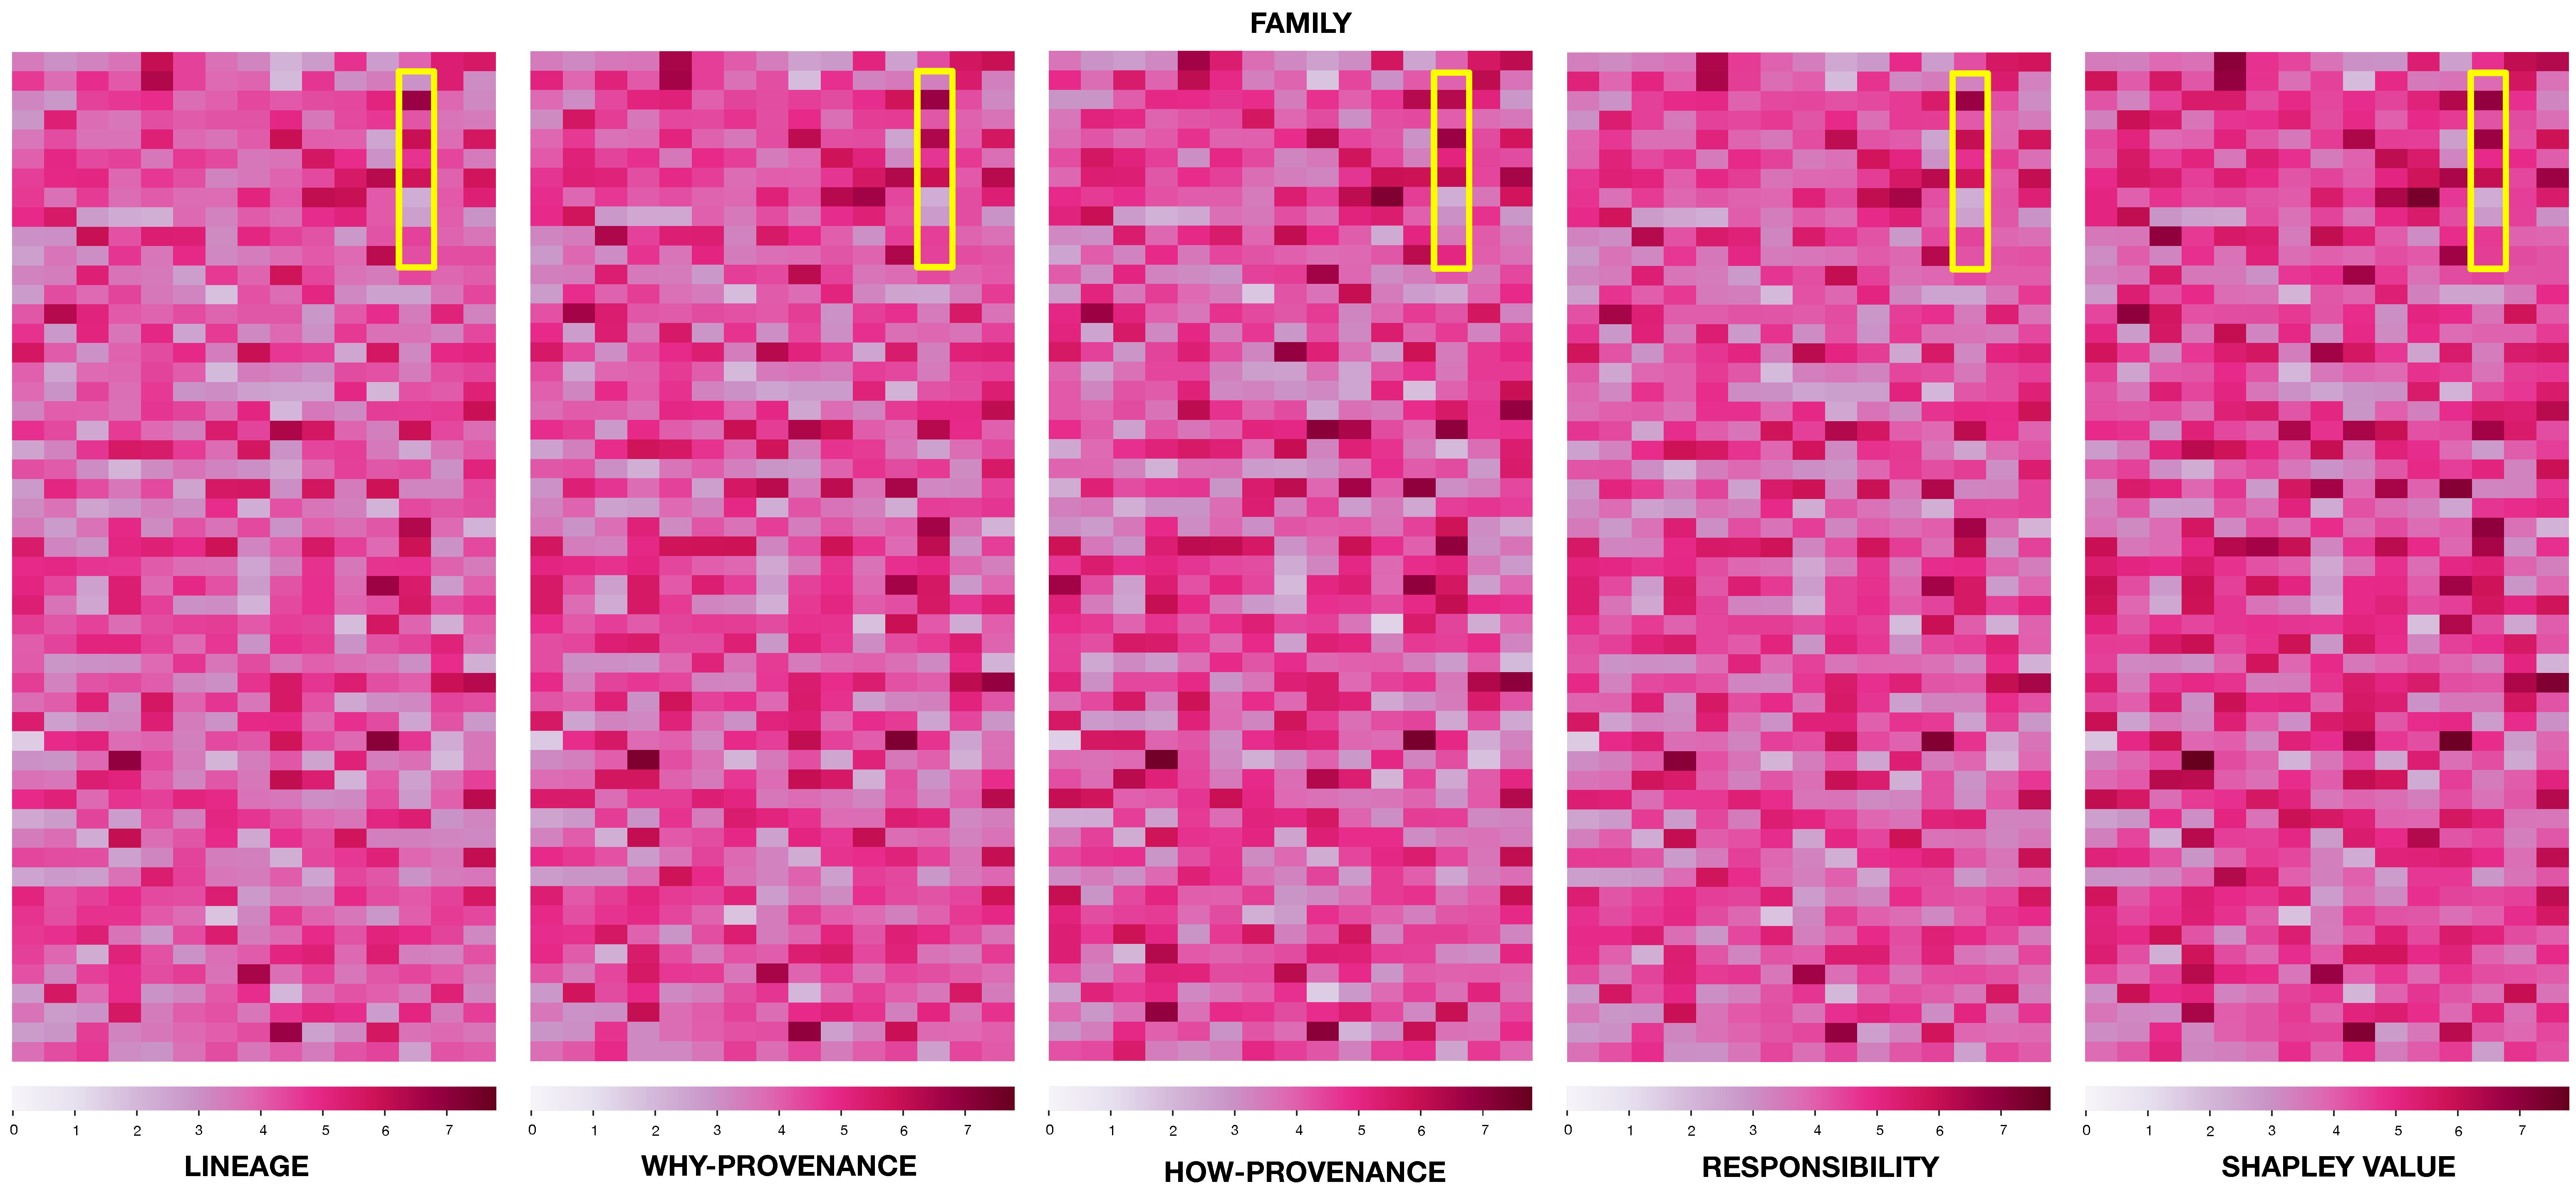
\includegraphics[width=1\textwidth]{figures/experiments/synthetic_comparison}
  \caption{Comparison of three DS on the same table \texttt{family} after the distribution computed using 10K synthetic and randomly generated provenance polynomials. The tuples in the blue rectangles are used as example in the discussion connected to Figure \ref{fig:comparison}.}
  \label{figure:comparison_on_synthetic_polynomials_2}
\end{figure}

\eat{
An example of such a synthetic provenance polynomial is:

{\footnotesize
\[
3 f_1^3 c2f_1^2 c_1^2 + 2 f_1 c2f_2^3 c_2^3 + 4 f_5 c2f_{17}^4 c_{18}^3
\] }
The corresponding why-provenance is: 
{\footnotesize
\[
\{ \{f_1, c2f_1, c_1\}, \{f_1, c2f_2, cf_2\}, \{ f_5, c2f_{17}, c_{18}\} \}
\] 
}
and corresponding lineage is: 

{\footnotesize
\[
\{f_1, f_5, c2f_1, c_1, c2f_1, c2f_2, c2f_{17}, c_1, c_2, c_{18} \}
\]}
 
 Using {\em how-provenance}, the distribution obtained from this sample polynomial is:

{\footnotesize
\[
f_1 = \frac{59}{315}, f_5 = \frac{1}{18}, c2f_1 = \frac{2}{21}, c2f_2 = \frac{2}{15}, 
c2f_{17}=\frac{2}{9} , c_1 = \frac{2}{21}, c_2 = \frac{2}{15}, c_{17} = \frac{1}{6} 
\]
}

Using {\em why-provenance}, the distribution is:

{\footnotesize
\[
f_1 = \frac{2}{9}, f_5 = \frac{1}{9}, c2f_1 = \frac{1}{9}, c2f_2 = \frac{1}{9}, 
c2f_{17}=\frac{1}{9} , c_1 = \frac{1}{9}, c_2 = \frac{1}{9}, c_{17} = \frac{1}{9} 
\]
}


Finally, with {|em lineage}, the distribution is:

{\footnotesize
\[
f_1 = \frac{1}{8}, f_5 = \frac{1}{8}, c2f_1 = \frac{1}{8}, c2f_2 = \frac{1}{8}, 
c2f_{17}=\frac{1}{8} , c_1 = \frac{1}{8}, c_2 = \frac{1}{8}, c_{17} = \frac{1}{8} 
\]
}
}



As an example of how the distribution strategies behave with these synthetic queries, consider tuple $f_5$ in Figure \ref{fig:syntheticDistributions}.
\rtwo{  This tuple receives the highest quantity of credit using responsibility-based distribution and less credit using, in order, lineage, the Shapley value, why- and how-provenance.
On the other hand, tuple $f_1$ is rewarded more by the Shapley value, then, in order, by why-provenance, how-provenance, responsibility, and finally lineage. 
This difference is explained considering the different role of the tuples in the generation of the output and the characteristics of the distributions.
Generally speaking, the more complex the distribution (e.g., the how-provenance), the more credit is given to tuples that are more frequently used or more critical in the production of the output. Depending on the situation, i.e. on the syntax of the query, the distributions may differ among them. 
Responsibility creates a ranking among lineage's tuples describing the importance of their role in generating the output. As such, the responsibility-based DS gives more credit to $f_1, f_5, c2f_{17}$ and $c_{18}$ due to their higher responsibility values. ``Importance'' is connected to their corresponding minimal contingency sets. For example, $f_1$ has a minimal contingency set (one of the many) $\{f_5\}$, with cardinality 1. On the other hand, $c_1$ has, as minimal contingency set (one of the many) $\{f_5, c_2\}$, with cardinality two. This means that $c_1$ is the ``least important'' amongst the tuples with minimal contingency sets of lower cardinality, and this is reflected in the different quantities of credit being distributed.} 

\rtwo{The Shapley value behaves similarly, but it rewards tuple $f_1$ the most and then $f_5$, $c2f_{17}$, $c_{18}$, and last all the other tuples of the lineage. Although both Responsibility and the Shapley value create a ranking of the tuples based on their role in the generation of the output, the corresponding functions behave differently due to the syntax of the query; for this reason each different distribution strategy highlights a slightly different aspect that can be considered as ``important'' when distributing the credit.}

Despite being synthetic, these provenance polynomials are realistic:  they can be obtained by any nested query with join and union operations that use the same tuple multiple times (in which case the exponents are larger than one), and the same combination of operations more than once (in which case the coefficients of monomials are larger than one). 

\paragraph{Results} The results of credit distribution on the \texttt{family} table using 10K randomly generated synthetic provenance polynomials are shown in
Figure \ref{figure:comparison_on_synthetic_polynomials_2}. 
We set the maximum value in the heat maps to the highest value reached by a tuple in all \rtwo{five} distributions (i.e., $7.7$, with the Shapley value-based DS). 

% \scream{DD: is the table described in this paragraph below helpful? If not, please delete.}
% \rtwo{As can be seen, the five strategies generate different credit distributions, indicated by the varying hues. We reported in Table \ref{table:in_detail} the values of credit assigned to the first five tuples of the table to show how these values actually differ between the five strategies. As can be seen, the strategies in these cases all behave differently. It is not even possible to identify a strategy that consistently rewards tuples more than the others, since this changes depending on the cases, reflecting the syntaxes of the polynomials being used.}

% \begin{table}[]
% \center
%   \caption{\rtwo{Quantities of credit given using the 5 DSs on the first five tuples of table \texttt{family} (tuples ordered by the \texttt{family_id} attribute of the table).}}
%   \begin{tabular}{|l|l|l|l|l|}
%   \hline
%  lineage & why & how & responsibility & Shapley \\
%   \hline
%  3.3603537 & 3.416667 & 3.5928571 & 3.3611114 & 3.425758 \\
%  4.4893217 & 5.111111 & 4.8620114 & 5.1752524 & 5.788059 \\
%  3.1333337 & 3.7888894 & 2.9106944 & 3.5000005 & 4.200001 \\
%  2.7972224 & 3.1111116 & 3.5601408 & 3.0055559 & 3.3305562 \\
%  3.4670746 & 3.8944445 & 3.7216337 & 3.8992426 & 4.31758 \\
%  \hline
%   \end{tabular}
%   \label{table:in_detail}
% \end{table}

\begin{table}[]
\center
  \caption{\rtwo{Results of the pairwise Kendall Tau confidence value on all the DSs on the \texttt{family} table (the p-vales are all below 0.05).}}
  \begin{tabular}{|r|l|l|l|l|l|}
  \hline
 & lineage & why & how & resp. & Shapley \\
  \hline
 lineage & 1.0 & 0.88 & 0.73 & 0.91  & 0.81 \\
why & 0.88 & 1.0 & 0.75 & 0.93 & 0.92 \\
 how & 0.73 & 0.75 & 1.0 & 0.74 & 0.74  \\
 resp. & 0.91 & 0.93 & 0.74 & 1.0 & 0.89 \\
Shapley & 0.81 & 0.91 & 0.74 & 0.89 & 1.0 \\
 \hline
  \end{tabular}
  \label{table:kendall_tau}
\end{table}
\normalsize


There is a certain amount of consistency between the strategies in that tuples which are highly rewarded by one strategy are also highly rewarded by the others. This shows that the four DSs consistently reward certain tuples more than others. 

\rtwo{Table \ref{table:kendall_tau} reports the pairwise Kendall $\tau$ correlation values\footnote{The Kendall's $\tau$ coefficient is a statistic used to measure the ordinal association between two measured quantities~\cite{Kendall1938new}. Intuitively, it is high between two variables when observation have a similar rank.} for the five DSs computed on the \texttt{family} table. As we see, there are certain DS that are correlated to others, such as lineage with why-provenance, responsibility and lineage, or responsibility and why-provenance. 
The others are mildly correlated, such as the Shapley valye with how-provenance, responsibility and how-provenance, or why-provenance and lineage with how-provenance. We see, therefore, that the DS based on how-provenance is the one that correlates the least with the other DSs.}

Note that lineage-based DS gives the least credit to tuples in the \texttt{family} table, indicated by an overall lighter hue. This is because the DS  distributes credit equally to all tuples appearing in the lineage. Since these queries also use two other tables, credit is distributed to tuples in those tables.

Moving to why-provenance-based DS, we see that more credit is given to tuples in the \texttt{family} table than with the previous strategy. This is because the DS considers the different ways that a tuple is used, e.g. in joins with other tuples. If the same tuple is present in more than one witness, it will draw more credit and take it from  other tuples in the witness basis. In this case, tuples in \texttt{family} drew more credit, taking it from tuples in the other two tables, due to the role that \texttt{family}  tuples played in the queries that were executed. 

Consider the how-provenance-based DS heat-map. %  in Figure \ref{fig:comparison}. 
As with why-provenance, more credit is typically given to tuples in \texttt{family} compared to lineage-based DS, since it recognizes the role of these tuples in the queries, and the overall hue is deeper.  
The two distributions appear similar, although on closer inspection, slight differences can be seen. 
This is because how-provenance also considers the frequency with which tuples are used, not only the ways in which they are used. Therefore, although the overall distribution is similar, there are small differences due to the presence of exponents and coefficients in the provenance polynomials, influencing the distribution of credit. 

\rtwo{The responsibility-based distribution strategy has a distribution that is also quite similar to the one provided by why-provenance (which is also visible from Table \ref{table:kendall_tau}). It is often the case, for example when the witnesses of the why provenance share one common tuple, that the two distributions behave similarly.} %As a consequence, the synthetic polynomials are at times such that the two distributions behave in the same way, or very similarly.} 

\rtwo{Finally, the heat-map reporting the distribution produced by the Shapley value is the one that, at a closer inspection, shows many differences. Although the tuples that receive the biggest quantities of credit are the same, the hue of this tuple is different. The Shapley value in certain circumstances differs greatly from the other DSs, thus showing its ability to weight differently the roles of the tuples.}

We note that the lineage-based DS gives an average credit of $3.92$ to each tuple in the table, while the DS based on why-provenance assigns $4.19$, how-provenance $4.18$, \rtwo{the one based on responsibility $4.13$, and the one based on the Shapley value $4.40$}. 
Moreover, lineage distributed a total of about $3121$ units of credit to the \texttt{family} table, why-provenance $3333$, how-provenance $3331$, while \rtwo{responsibility assigned $3290$, and the Shapley value $3505$. Thus, the Shapley value is the method that accumulates the highest quantity of credit in this table.} 
%That is, the DS based on why-provenance assigns on average $50\%$ more credit to the \texttt{family} table than the strategy based on lineage.
%\scream{GMS: It could be interesting (and simple to do) to report a number to quantify the amount of credit distributed by the three strategies, so that we can say that how-provenance distributes, say, 20\% more credit than lineage or so. The number could be the sum of each tuple credit or its average. Make sense? Not sure if this is just useless info.} 


To better understand the differences between DSs, in the next subsection we consider the accrual of credit over time.  In doing so, we will focus on the ten tuples shown within the large yellow rectangles in Figure \ref{fig:comparison}.  Each small rectangle within a large yellow rectangle is a tuple, and we number them from $1$ (top) to $10$ (bottom). 
\rone{These ten tuples were cherry-picked because they allow us to see the evolution of the distribution of credit through time. There are other tuple sets that could have been selected driving us to the same considerations.}

\eat{
 Note that tuples 2, 7, 8, and 9 are awarded less credit than in either the lineage- or why-provenance strategies, whereas tuples 1 and 3 receives more credit than either of the other two strategies. 
 
However, the distribution does not reward tuple 2 in the same way. Also tuples 7, 8, and 9 that appear to be rewarded heavily in the why-provenance-based DS here are contain lower quantities of credit. Vice-versa, tuple 3 is much higher in credit with respect to what happens with the why-provenance-based DS.
This is due to the fact that this DS is even more sophisticated, since it uses all the information contained in the provenance polynomials. 
In this case, a tuple as 3 is able to attract even more credit than before. However, other tuples, such as 2, 7, 8, and 9 receive now less credit, since they role appears to be less determinant once the full information from the polynomials is taken into considerations. }
\eat{even more sophisticated, and can be taken into consideration when a user wants to distribute credit with a higher level of sensibility.}
%\textbf{ $\leftarrow$  Gianmaria: This is not clear and I suggest a rewriting of this paragraph.}

%%%%%%%%%%%%%%%%%%

\subsection{Credit accrual over time} 
Since credit accrues over time, we simulate the passage of time by varying the number of queries executed, and look at the ``snapshots" of credit for each of the strategies using synthetic queries.  The results are shown in Figure \ref{fig:comparison}.

\begin{figure}[h!]
\centering
  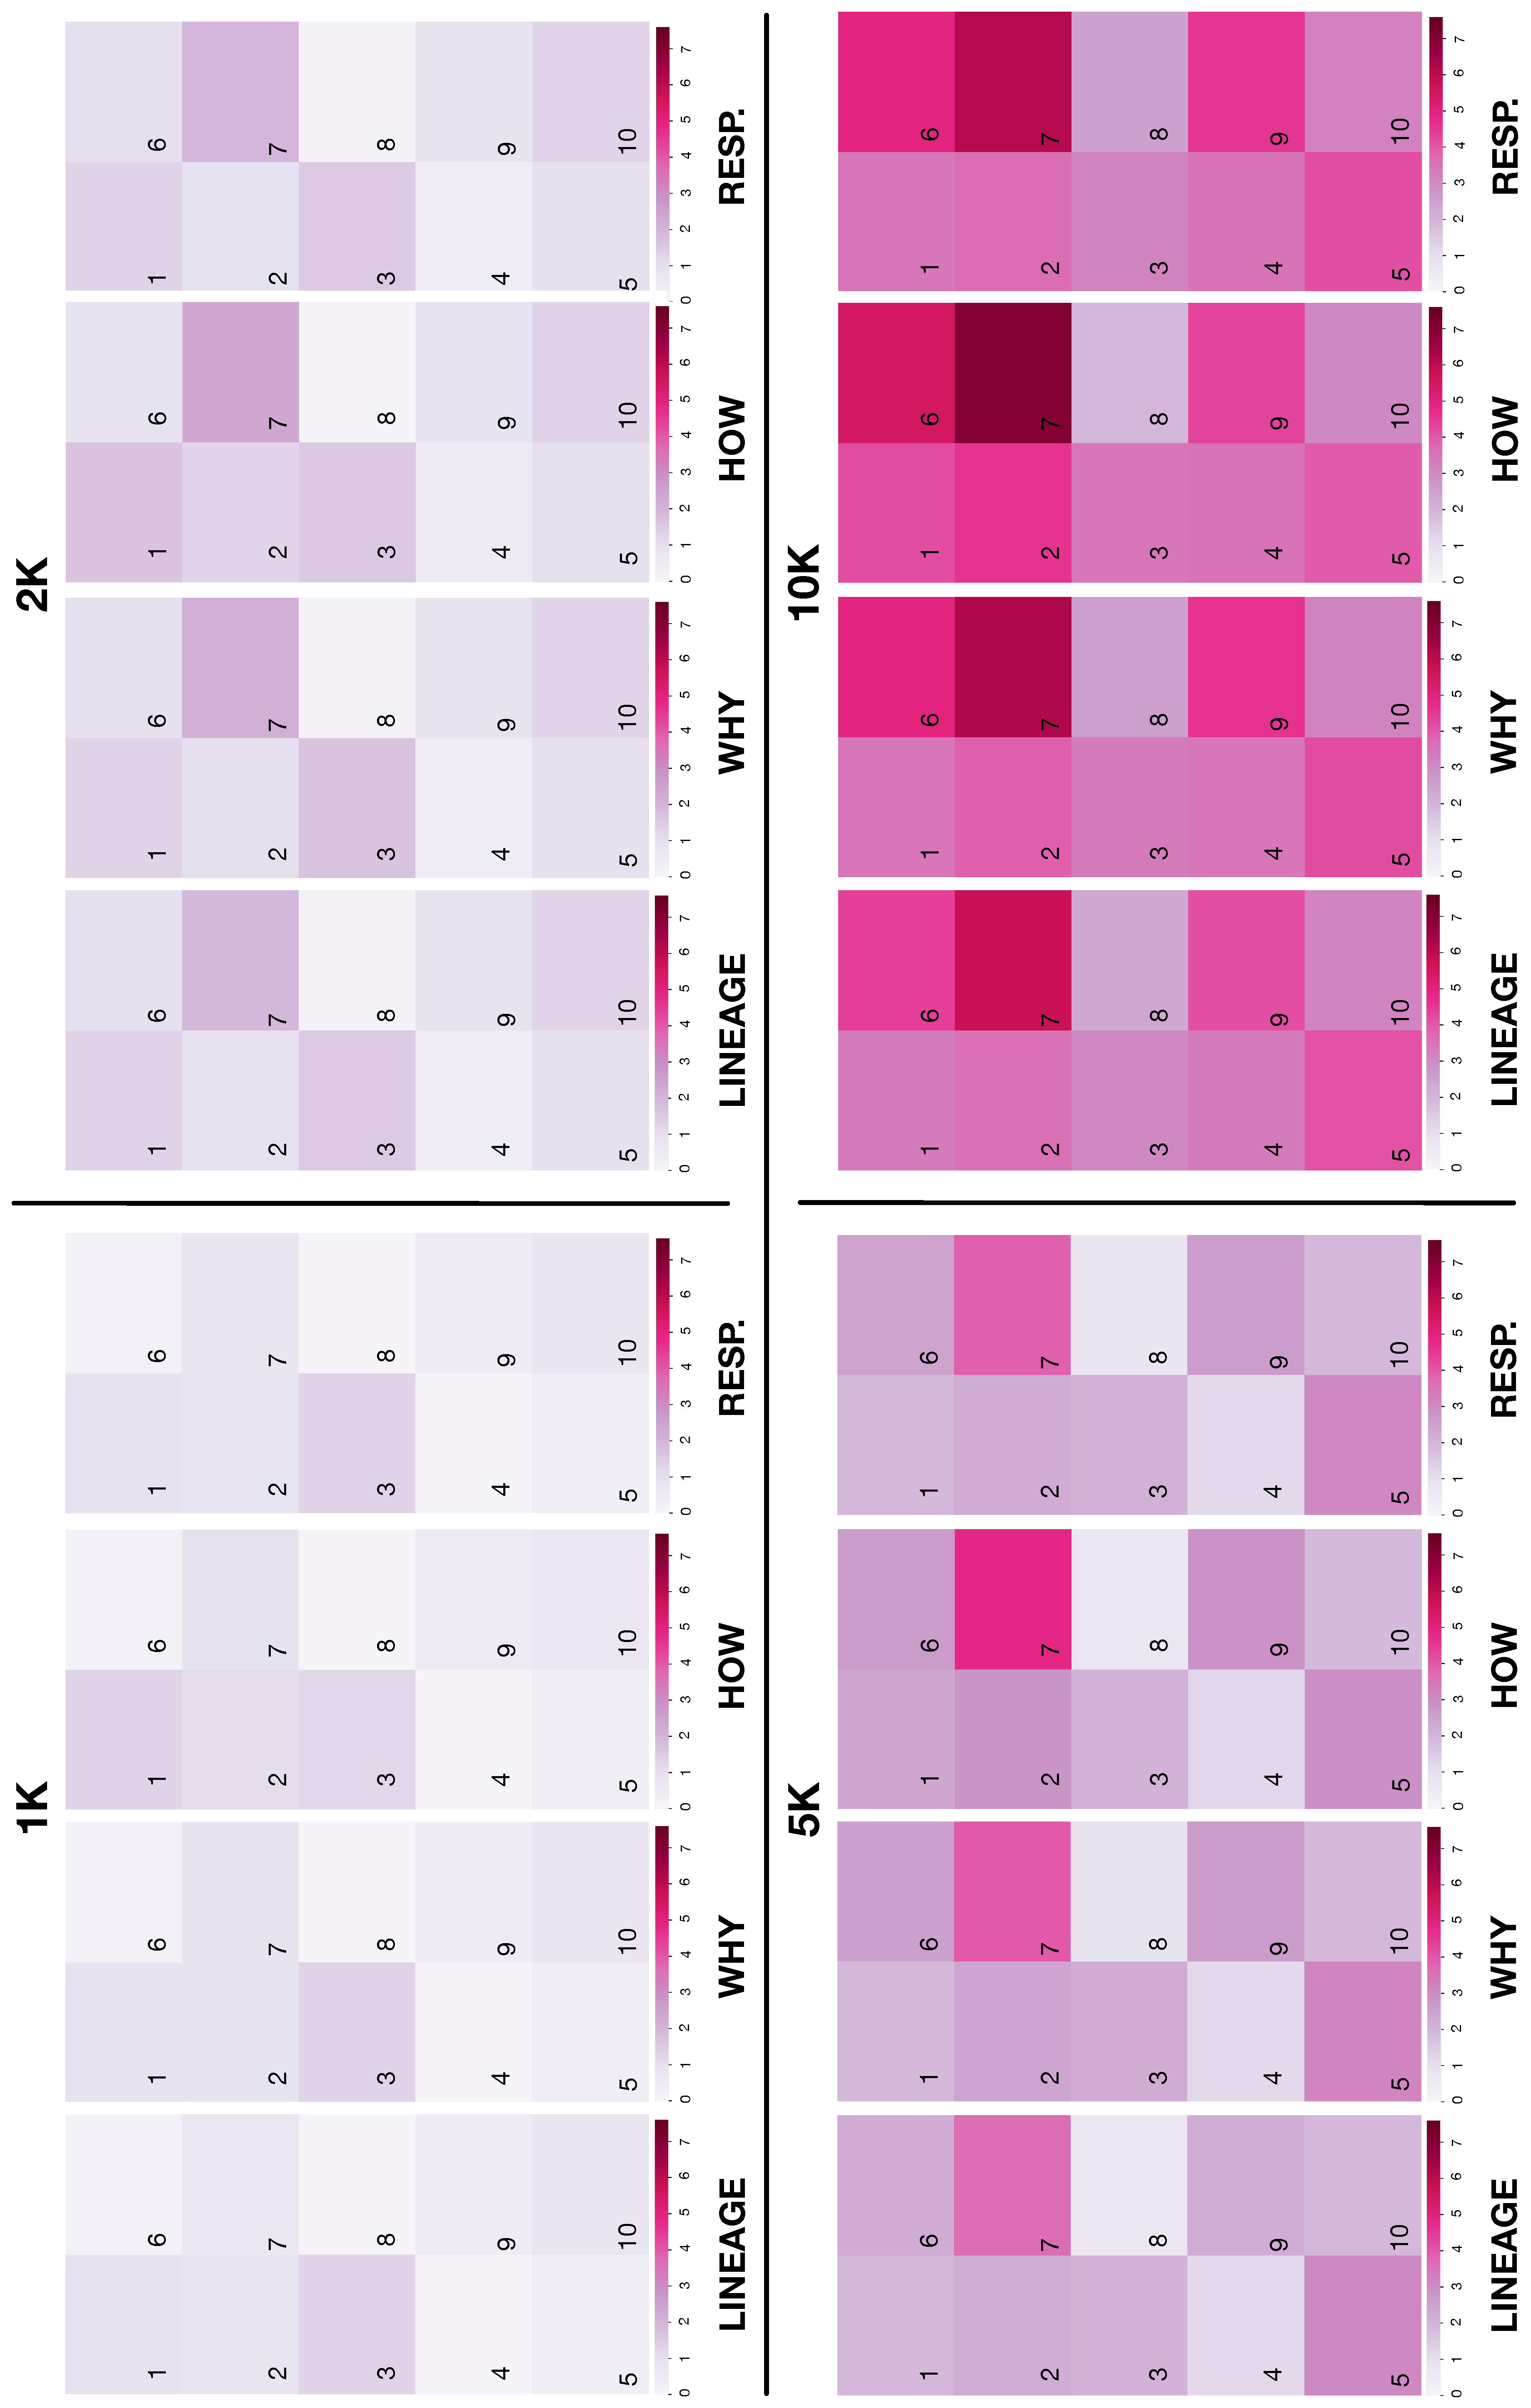
\includegraphics[width=.60\textwidth]{figures/experiments/comparison}
  \caption{\rtwo{Comparison of the distribution of credit performed by the \rtwo{five} DSs on a subset of 10 tuples taken from the \texttt{family} table, simulating the passing of time. The number at the top of each group of heat-maps represents the number of polynomials whose credit has been distributed.}}
  \label{fig:comparison}
\end{figure}

In this figure, four groups of heat-maps are shown. Each group represents a ``snapshot'' taken %during an incremental accumulation of credit on the database 
after 1K, 2K, 5K and 10K provenance polynomials have been considered for credit distribution.  
The ten tuples in each heat-map  %from the \texttt{family} table, and
are those  highlighted in the \rone{yellow} boxes of Figure \ref{figure:comparison_on_synthetic_polynomials_2} from the \texttt{family} table.  


The polynomials used are the same as the experiment of the previous section. The range of credit in each map goes from 0 (no credit) to $7$ (the maximum quantity of credit reached -- using how-provenance -- on one of the tuples of the considered window at the ``snapshot'' with 10K queries). The color hue of the legend, as can be seen, still ranges from $0$ to $7.7$.

%\scream{I feel that this section is going into too much detail.  We should just get the big idea across.  I have "eaten" most of this text and tried to pull out the highlights. Don't bring up things unless you can explain them, or are trying to make a point.  The other problem is we can't really say why tuples wax and wane in overall credit -- it depends on the queries, which we don't go into (or want to go into).}

By the end of 1K queries, credit differentials between tuples as well as between strategies can be seen.  For example, tuple 3 is usually rewarded the most credit by all five strategies. 
\rtwo{Moreover, it can be seen that tuples $1$ receives a higher quantity of credit when how-provenance is adopted, showing how this form of provenance behaves differently from the others in this context}.
Moving to $2K$ queries, it is possible to see that tuple $3$ and $7$ are still the most rewarded by the strategies.

By the end of 5K queries, tuple $7$ emerges with the highest value of credit with all five DSs, a position which is strengthened with 10K queries. Moreover, with the passing of time, tuple $3$ ceases to be one of the most rewarded ones and new tuples, such as $6$ and $9$, emerge as being particularly rewarded at 5K, while at 10K tuples $6$ and $7$ are the most rewarded from the distributions.
This is because tuple $7$ is used several times within queries being executed, which is rewarded strongly by why- and how-provenance.
\rtwo{We also note that the responsibility-based distribution confirms its trend of being similar to why-provenance, although not identical. This is more evident at step 10K, where tuple 7 is slightly less rewarded using responsibility ($6.12$) with respect to why-provenance ($6.24$). 
The responsibility that rewards the more tuple $7$ is the one based on how-provenance (credit $7.03$), followed by the Shapley value (credit $6.64$).
This is due to the fact that tuple $7$ had, among some of the polynomials being used for the experiments, a high responsibility but it did not appear in all witnesses. This changed slightly the distribution.}


While the relative value of credit ``positions" of tuples within a DS strategy depends on what queries are being executed, the important thing to notice is the difference between the DSs over time:  overall, lineage gives less credit to tuples in the \texttt{family} table than the other strategies since credit is shared with tuples in other tables.
The other strategies recognize the more important role being played by the \texttt{family} tuples than those in the other tables.
\rtwo{The differences between why- and responsibility-based DS are, for the most times, negligible.} 
The differences between the why- and how-provenance-based DSs are also relatively minor in most cases. However, there are certain situations in which the role of a tuple is particularly critical in a query, and in this case the difference in the value of credit assigned is notably higher for how-provenance \rtwo{and the Shapley value}, as we saw with tuple 7 in the example of Figure \ref{fig:comparison}. 


\eat{
Focusing on the 1K and 2K groups, we see that credit distribution by the three DS are very similar, but that there are small differences.
We note that, in the 1K group, tuple 4 has the highest value of credit within all three strategies. Moving to the 2K group, tuple 4 still has the highest value of credit, although it has the highest value with the why-provenance DS; the other two strategies rewarded it less. 
In contrast, why-provenance and how-provenance rewarded tuples 2 and 3 more than the strategy based on lineage. 
Tuple 5 appears to be rewarded more by why-provenance and less by how-provenance, and even less by lineage. 
\scream{I don't understand what a "lower value of polynomial" is?  Do you mean lower number of queries?}
This shows that, even with these lower values of polynomials, that the strategies may differ and reward certain tuples more than others. 
We see the tendency of the lineage DS to reward tuples in this table less than the other strategies, since it does not take into consideration their importance. 
Instead, the DS based on why-provenance rewards more tuples like 4 and 5 (values 2 in both cases). 
The same can be said of the strategy based on how-provenance. However, in this case, tuples 4 and 5 are rewarded a little less (with credit values of 1.9 and 1.5 respectively). This is due to the fact that how-provenance contains more information. Thus, this DS rewarded more other tuples in the other used tables. Viceversa, tuples 2 and 3 are rewarded more by how-provenance DS (values 1.5 and 1.6) that the why-provenance DS (value 1.3 in both cases), due to the fact that their roles in the polynomials are more important.  
}

\eat{
Moving to the 5K group, we see how credit was accumulated on the tuples. Now tuple $2$ is the one with the biggest quantity of credit in this window. This shows how credit is able to track how the importance of tuples changes over time. 
In this group we see of it is more evident the difference between the distribution based on lineage and the other two strategies. The why-provenance and how-provenance based DSs appear to work similarly, that is to give similar values of credit to the same tuples. 
We can still see differences, for example on tuples like 8 and 6, that are more rewarded by the DS based on lineage.}

\eat{
Similar observations can be seen for the 10K group. We see how tuple 2 is still highly rewarded by all three provenances. In the case of lineage, however, it is at the same level with tuples 3, 4, and 8, while the other two strategies reward it the most. 
Once again we see the DSs based on why- and how-provenance operate similar distributions (we still note differences of few decimals between the values assigned to the tuples). However, it is still possible to see how tuples like $9$ are more rewarded by one DS, in this case the how-provenance one, than the other. 
This shows how the last two DS operate in a similar way. The differences between the credit assigned to the same tuple is of few decimals between the two strategies in most of the cases. However, there are certain situations when the role of a tuple is particularly critical in a query. This information is captured by the provenance polynomial, and this is why in certain cases the differences in the credit assigned to one tuple is notably different between the two strategies.  
}


To sum up, the DS based on lineage is sufficient to highlight which tuples in the database are used by a query, and distributes credit equally to these tuples. The resulting distribution rewards tuples that are used by more queries, but does not reward how many times tuples are used in the same query.  
However, a DS based on why-provenance, \rtwo{responsibility, Shapley value} or how-provenance may be better if the queries are complex, since they reward more tuples that have a critical role in generating the output. %These two DS are sensitive than the DS based on lineage (and the DS based on how-provenance is more sensible than the one based on why-provenance). 
\eat{Using the why-provenance and how-provenance DS, it is possible to change the distribution of credit to the tuple, rewarding more the tuples that have a more critical role in generating the output. The distribution based on how-provenance is most of the times similar to the one based on why-provenance. 
However, in certain instances, it differ from the other one due to the specific role of a tuple, an information that is present in the provenance polynomial but lost in the witness basis. }
In particular, these \rtwo{four} DSs may be useful for finding ``hotspots'' in the database based on the role of tuples, with the how-provenance-based and Shapley value-based DSs being preferable if a higher sensitivity to the role of a tuple in queries is required. 

%In particular, the DS based on why-provenance rewards more the tuples that are used in different ways by queries (i.e. are members of more witnesses). The DS based on how-provenance also takes into consideration how many times a tuple is used, adding even more sensibility to the distribution. 
%One may choose one other the other depending what are the aspects he wants to highlight in the data.

%%%%%%%%

\subsection{Credit vs Citations}

\begin{figure}[]
\centering
  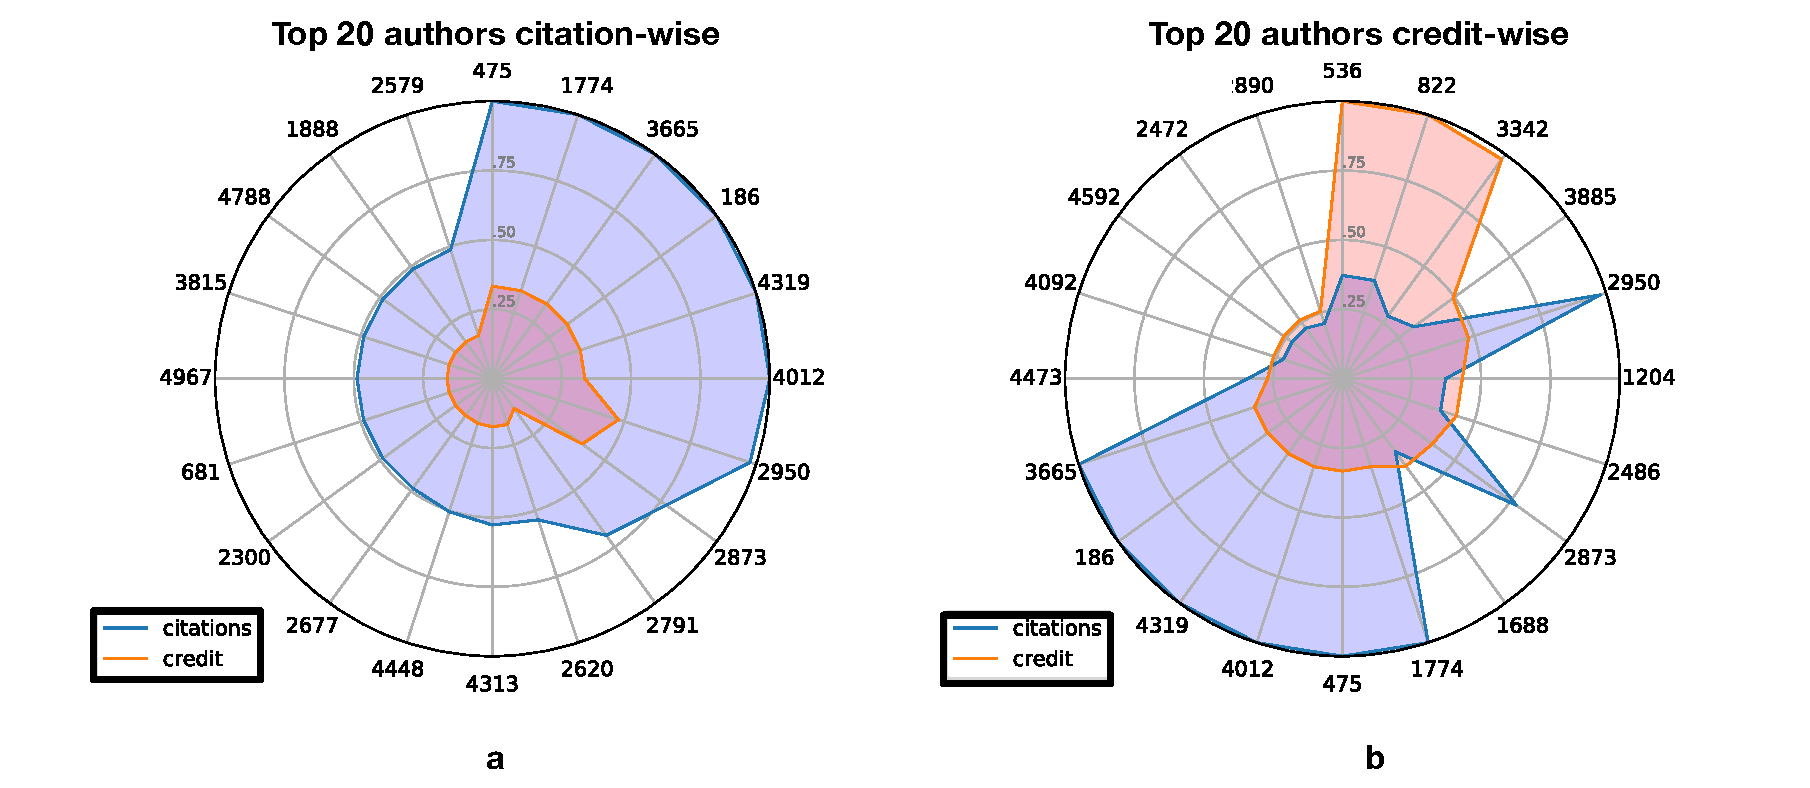
\includegraphics[width=1\textwidth]{figures/2_radars}
  \caption{Radars presenting the top 20 authors citation-wise and credit wise, together with their (normalized between 0 and 1) values of citations and credit.}
  \label{figure:2_radars}
\end{figure}

In the last set of experiments, we compare traditional citations to the proposed credit distribution strategies to see the difference in reward for data authors and curators.  
\textcolor{correction}{Using both real-world and synthetic queries, we distribute credit to the authors responsible for the data under the different strategies. Our results show that credit rewards authors of data that is cited fewer times, but that has a higher impact on the query results.} 
%\scream{Reprise from the intro exactly what this is doing and why.}

\textcolor{correction}{To do so, we need to identify a set of authors and queries that cite data curated by them.}  
Considering GtoPdb, each target family page has a list of curators, representing the people who are co-creators and curators of the data comprising the page. This list can be obtained using the last query shown in Figure \ref{figure:family_structure}. 
Each time a target family page is cited, we assign one {\em citation} to each author associated with the page.  The authors also receive {\em credit} in the amount assigned to the data used by the query to construct the webpage, equally divided between the authors of the webpage.


\paragraph{Results: Real-world queries}
As described in Section \ref{sec:real_world_queries}, we consider real-world queries taken from papers published in the BJP which reference webpages in GtoPdb.
Since for these queries there is no difference in the distribution of credit between the DSs, only one value for credit is used.
%given in Figure \ref{figure:2_radars}. \eat{As we said, each time a webpage is cited, the authors of that webpage receive one citation, and also receive a quantity of credit that is equal to the credit assigned to the data and generated from the citation, equally divided among them.} 

The results are shown in the radar plots of Figure \ref{figure:2_radars}, in which each number on the outer circle (e.g. 475, 1774 and 3665) represents an author (id) and the blue (red) line represents the normalized value of credit generated by citations (credit), respectively. The first radar plot,
Figure \ref{figure:2_radars}.a, shows the top 20 authors in terms of {\em citations}, ordered in a clockwise direction, whereas Figure \ref{figure:2_radars}.b orders the authors based on {\em credit}. 
Comparing the author ids used in the outer circles of these two plots, it can immediately be seen that the ``top authors'' are very different using these two metrics, although there is some overlap (for example, authors 1774, 475, and 4012). 

%\scream{I don't understand what you are trying to say here.  Rewrote, putting old in eat in case I am wrong.}
Diving a bit deeper to focus on the red and blue areas in each of the plots reveals that there is a significance difference between citations and credit:
The top 20 authors in terms of citations do not have the highest values of credit (Figure \ref{figure:2_radars}.a).  Conversely, the authors with the highest values of credit do not necessarily have a large number of citations (Figure \ref{figure:2_radars}.b).
\eat{This is due to the fact that certain citations are more ``valuable'' in terms of credit, i.e. an author receive more credit from his/her citations, even if fewer, than other authors. This, in turns, happens because certain citations generate more credit than others. 
So, for example, author 536 presents the highest value of credit, although he is not even in the top 20 authors in terms of citations. This means that he receives much more credit from his relatively few citations than author 475. }
For example, author 536 has the highest value of credit, but is not even in the top 20 authors in terms of citations. This means that authors like 536, 822, and 3342 in Figure \ref{figure:2_radars}.b receive much more credit from their relatively few citations than authors like 475, who receives the largest number of citations.
That is, the data underlying certain webpages is more ``valuable'' in terms of credit than a citation to the webpage.  

\eat{Given how we prepared our experiments, the citations whose query produce more tuples, are also the ones that generate more credit, since we assumed that each output tuple carries credit $1$. Thus, the authors of the data returned by these queries are the ones that will receive more credit from these citations. Also, the authors that collaborated with fewer people will also receive a biggest share from the equal subdivision of credit. }

The reason for the difference between citation and credit is partly due to the experimental setup:  each output tuple carries a credit of $1$, and there can be many tuples used to generate a webpage.  Thus a webpage that is created from more tuples will have a higher credit value than one created from fewer tuples. Furthermore, authors who collaborated with fewer people will receive a biggest share of the equally divided credit.  However, all authors will receive a citation of one.

Credit distribution therefore rewards authors differently than traditional citations: an author who has curated larger quantities of cited data and collaborated with fewer co-authors, will receive larger quantities of credit. Thus, credit rewards them for their larger contribution to the database. 

%In other settings, where the quantity of credit can be computed considering different criteria, such as the impact of the cited data in the citing paper, credit distribution can help to identify with even deeper precision the data and the authors that contributed more to the scientific impact in the context defined by the considered citations.

%\scream{I "ate" the final paragraph. I didn't understand what other strategies you are talking about and thought it was more more in keeping with "future work"?}

%\begin{figure}[t]
%\centering
%  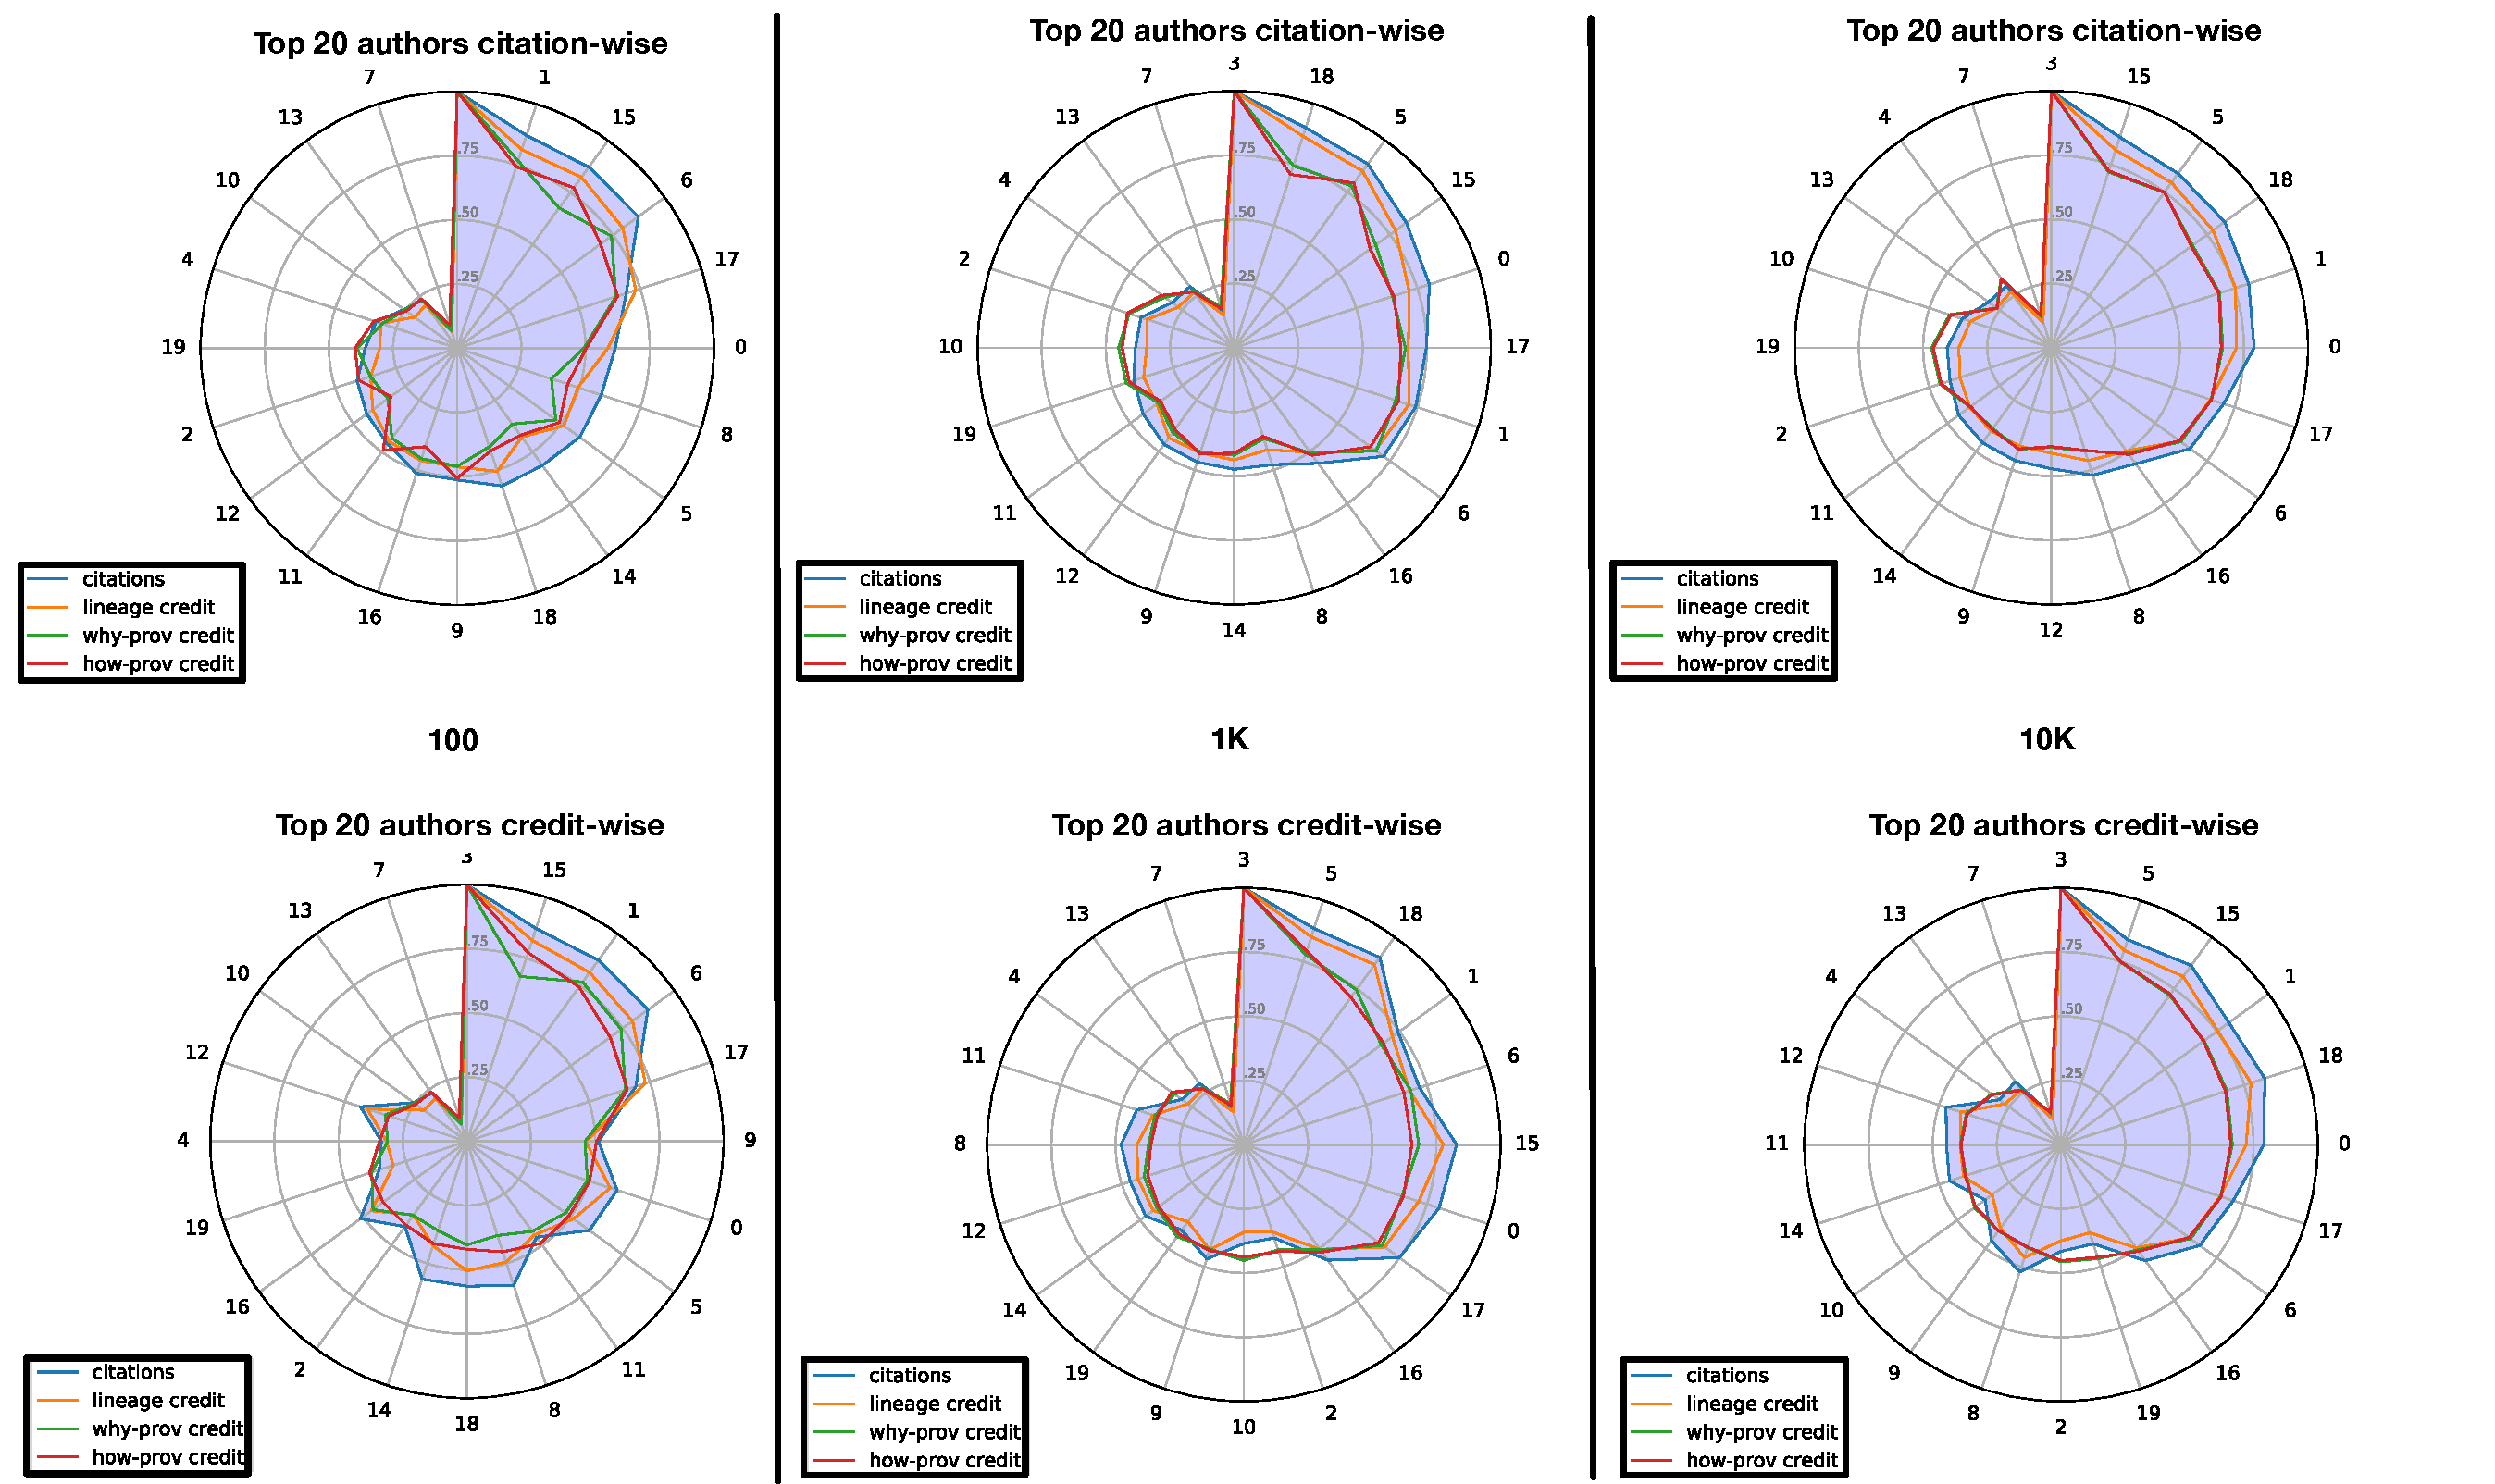
\includegraphics[width=1\textwidth]{figures/3_radars}
%  \caption{Radars presenting 20 authors ordered citation-wise and credit-wise, together with their (normalized between 0 and 1) values of citations and credit, through the execution of different numbers of polynomials (100, 1K, and 10K). The radar plots ordered by credit consider the credit assigned by the DS based on how-provenance.}
%  \label{figure:3_radars}
%\end{figure}

\begin{figure}[t]
\centering
  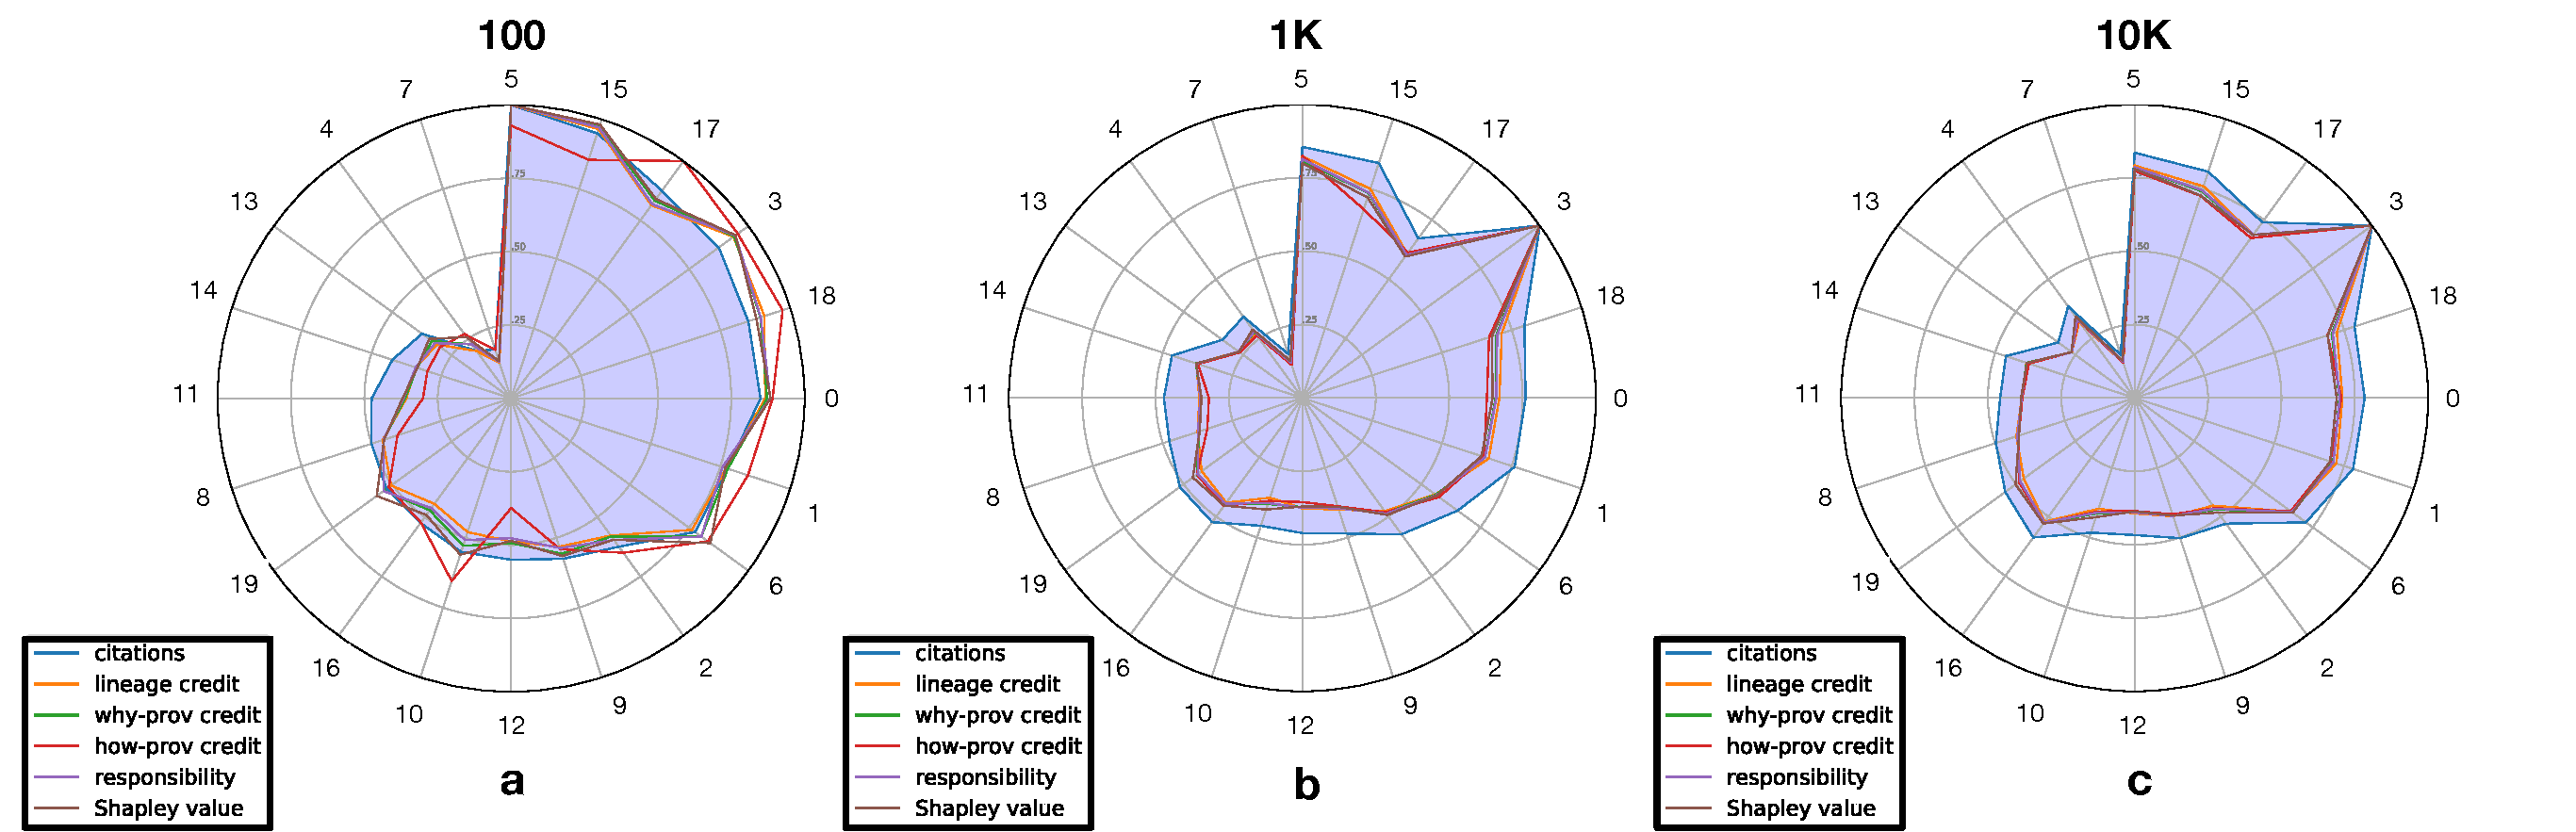
\includegraphics[width=1\textwidth]{figures/radar}
  \caption{
\rtwo{  Radars presenting the 20 synthetic authors with corresponding citation and quantities of credit distributed through the 4 DSs (all values normalized between 0 and 1) through different numbers of polynomials (respectively, 100, 1K and 10K). 
  The order is the one defined by figure a, i.e. descending order of citations  obtained from 100 polynomials.}}
  \label{figure:3_radars}
\end{figure}

\paragraph{Results: Synthetic queries}
We used the same synthetic polynomials described in Section \ref{sec:synth_queries}, and we distributed credit with the first $100$, $1K$, and $10K$ of them.
Since these polynomials are created by randomly selecting tuples from three tables, they usually correspond to a set of data curated by  authors who, in reality, did not collaborate. To make the size of the author set more realistic, we therefore created $20$ synthetic authors, and randomly assigned one author to blocks of consecutive tuples in the database, with the size of each block varying between $10$ and $40$, to simulate different quantities of work performed by an author. 
Every time an author appears as curator of one or more tuples used in a polynomial, we assign them one citation.  
They also receive four kinds of credit, each one using a different DS.

Figure \ref{figure:3_radars} shows three radar plots, one for the results obtained with 100 polynomials, one with 1K polynomials, one with 10K polynomials.  
Each plot shows the top 20 authors in terms of citations (hence the authors and clockwise ordering is the same in each of the plots), and additionally shows the the normalized values of citation (blue line), lineage-based credit (yellow line), why-provenance-based credit (green line), how-provenance-based  credit (red line), \rtwo{responsibility-based credit (violet line), and the Shapley value-based credit (brown line)}. 

As can be seen, given the synthetic nature of the queries, the correlation between the number of citations and the quantity of credit assigned to the authors appears to be a much stronger than with the real-world queries of Figure~\ref{figure:2_radars}. In fact, for Figure \ref{figure:3_radars}.a  the linear correlation between the citation number and all four types of credit is always above 0.94 with p values in the order of 3e-8.
\eat{Nonetheless, it can still be seen that credit does not always follow the citation count. }
The credit distributed via lineage is closest to  the number of citations (a linear correlation of 0.99, p value of 2e-16 in Figure \ref{figure:3_radars}.a), while the other three types of credit behave slightly differently (a linear correlation of around 0.95 or above in all other four cases in Figure \ref{figure:3_radars}.a).  
Similar observations can be made for Figure \ref{figure:3_radars}.b and \ref{figure:3_radars}.c.

What these figures show is that, in certain cases, authors who do not have a large number of citations receive more credit than others, as for example authors 17, 18 and 10 in Figure \ref{figure:3_radars}.a, 
%or author 19 in Figures \ref{figure:3_radars}.b and \ref{figure:3_radars}.c, 
and especially when credit is distributed using how-provenance.
This again shows how credit gives a different perspective on the role of data and authors by going beyond the limitations of traditional citations.  

It is worth noting that, when scaling up to $1K$ and $10K$ polynomials, the credit distributions  become almost identical  
\eat{We note that, although not exactly overlapping, the values of credit assigned to the authors by those DS become quite similar with these higher quantities of polynomials, suggesting a sort of equivalence between the two DSs in this case, at least in the task of rewarding authors} (the linear correlation for the values of Figure \ref{figure:3_radars}.c is more than 0.99 with a p-value of 1.32e-32). This is consistent with what we observed in Figure \ref{figure:comparison_on_synthetic_polynomials_2}.


\eat{
\subsection{Execution time}
The last experiment compared the time required to calculate the credit distribution for the three strategies. The results are shown in Table \ref{table:times}.  

\begin{table}[hbt]
\centering
  \begin{tabular}{| l |c | c | c | c ||}
  \hline
    \# of polynomials  & lineage & why-prov. & how-prov. \\
    \hline
    100 & 226.6 ms & 192.0 ms & 185.5 ms \\
    200 & 431.2 ms & 392.2 ms & 403.2 ms \\
    500 & 1.013 s  & 934.2 ms & 881.8 ms \\ 
    1K  & 2.041 s  & 1.934 s  & 1.744 s  \\
    2K  & 3.773 s  & 3.491 s  & 3.510 s  \\
    5K  & 8.992 s  & 8.653 s  & 8.889 s  \\
    10K & 17.10 s  & 16.84 s  & 16.84 s  \\
    20K & 34.59 s  & 35.30 s  & 39.70 s \\
    100K & 3.289 min & 3.442 min & 3.652 min \\
    1M  & 35.91 min & 34.87 min & 37.91 min \\
    \hline
  \end{tabular}
  \caption{The times required to perform the three DS for different number of synthetic polynomials.}
  \label{table:times}
\end{table}

\scream{Perhaps you should plot these using lines?  It is not easy to see that it grows linearly.  Also, why is linage almost always slower than the why- and how-provenance?  How was the experiment performed?}
As can be seen, the execution time grows linearly with the number of polynomials that are submitted to the system. When there are a large number of polynomials (1M), the time required by the DS based on lineage and why-provenance is slightly less than the time needed for the DS based on how-provenance. This is due to the increased complexity of the how-provenance calculation.  \scream{How significant is the difference?}
We note that, since we created these polynomials on-the-fly, these values do not include the time required to compute the provenances.
Therefore, just taking into account the time required to distribute credit, the three DS are roughly the same in terms of performance. 
\scream{This seems a bit of a contraction to the previous claim of "increased complexity".}
Only when there are a large number of complex polynomials do lineage and why-provenance  become preferable to how-provenance in terms of execution time, but coming at the cost of a less equitable credit distribution strategy.
}


%\subsection{Discussion}
%
%In the previous sections we showed, through the use of different experiments, the behavior of credit and its distribution with the use of different DS. 
%It appeared that, in the case of SPJ queries, the three distributions behave in the same way on GtoPdb. 
%
%Using synthetic polynomials, we showed how the three DS actually behave differently, in particular with the passage of time, i.e. when more and more polynomials are processed. 
%The three DS are all effective ways to distribute credit, and there is not one distribution that is preferable to the other all the time. It all depends on the needs of the users. 
%
%Lineage is to be preferred when users only want to find tuples that are used in a database by queries applied to this database. With the accumulation of credit coming from many queries, the DS based on lineage is also able to create ``hotspots'' among the tuples of the relational database.
%However, lineage rewards equally the tuples used by a query.
% 
%Why-provenance is more versatile when users also want to consider how many ways a tuple is used; thus, in a way, its \emph{versatility} inside the queries that used it.
%Finally, how-provenance also counts how many times a tuple is used, its \emph{frequency} in the computation of a query. 